\documentclass[a4paper]{article}
\usepackage{verbatim}
\usepackage{tikz}

\begin{document}

\begin{center} 
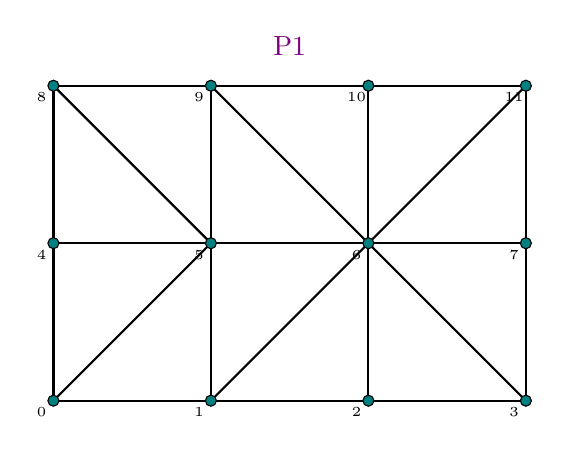
\begin{tikzpicture} 
\node[violet] at (3,4.5) {P1}; 
\draw[thick] (0,0) -- (6,0) -- (6,4) -- (0,4) -- cycle; 
\draw[thick] (0,2) -- (6,2) ; 
\draw[thick] (2,0) -- (2,4) ; 
\draw[thick] (4,0) -- (4,4) ; 
\draw[thick] (0,0) -- (2,2) -- (0,4) ; 
\draw[thick] (2,0) -- (4,2) -- (2,4) ; 
\draw[thick] (6,0) -- (4,2) -- (6,4) ; 
\draw[black,fill=teal] ( 0.000000 , 0.000000)     circle (2pt); 
\node[] at ( -0.150000, -0.150000 ) {\tiny 0 }; 
\draw[black,fill=teal] ( 2.000000 , 0.000000)     circle (2pt); 
\node[] at ( 1.850000, -0.150000 ) {\tiny 1 }; 
\draw[black,fill=teal] ( 4.000000 , 0.000000)     circle (2pt); 
\node[] at ( 3.850000, -0.150000 ) {\tiny 2 }; 
\draw[black,fill=teal] ( 6.000000 , 0.000000)     circle (2pt); 
\node[] at ( 5.850000, -0.150000 ) {\tiny 3 }; 
\draw[black,fill=teal] ( 0.000000 , 2.000000)     circle (2pt); 
\node[] at ( -0.150000, 1.850000 ) {\tiny 4 }; 
\draw[black,fill=teal] ( 2.000000 , 2.000000)     circle (2pt); 
\node[] at ( 1.850000, 1.850000 ) {\tiny 5 }; 
\draw[black,fill=teal] ( 4.000000 , 2.000000)     circle (2pt); 
\node[] at ( 3.850000, 1.850000 ) {\tiny 6 }; 
\draw[black,fill=teal] ( 6.000000 , 2.000000)     circle (2pt); 
\node[] at ( 5.850000, 1.850000 ) {\tiny 7 }; 
\draw[black,fill=teal] ( 0.000000 , 4.000000)     circle (2pt); 
\node[] at ( -0.150000, 3.850000 ) {\tiny 8 }; 
\draw[black,fill=teal] ( 2.000000 , 4.000000)     circle (2pt); 
\node[] at ( 1.850000, 3.850000 ) {\tiny 9 }; 
\draw[black,fill=teal] ( 4.000000 , 4.000000)     circle (2pt); 
\node[] at ( 3.850000, 3.850000 ) {\tiny 10 }; 
\draw[black,fill=teal] ( 6.000000 , 4.000000)     circle (2pt); 
\node[] at ( 5.850000, 3.850000 ) {\tiny 11 }; 
\end{tikzpicture} 
\end{center} 


\begin{tiny}
\verbatiminput{iconV_P1.ascii}
\end{tiny}


%--------------------------------
\newpage
\begin{center} 
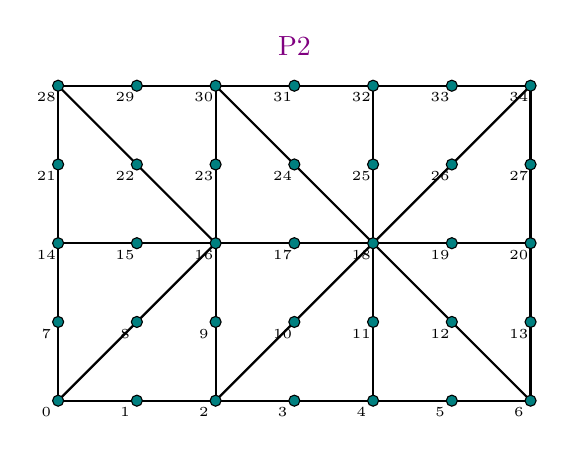
\begin{tikzpicture} 
\node[violet] at (3,4.5) {P2}; 
\draw[thick] (0,0) -- (6,0) -- (6,4) -- (0,4) -- cycle; 
\draw[thick] (0,2) -- (6,2) ; 
\draw[thick] (2,0) -- (2,4) ; 
\draw[thick] (4,0) -- (4,4) ; 
\draw[thick] (0,0) -- (2,2) -- (0,4) ; 
\draw[thick] (2,0) -- (4,2) -- (2,4) ; 
\draw[thick] (6,0) -- (4,2) -- (6,4) ; 
\draw[black,fill=teal] ( 0.000000 , 0.000000)     circle (2pt); 
\node[] at ( -0.150000, -0.150000 ) {\tiny 0 }; 
\draw[black,fill=teal] ( 1.000000 , 0.000000)     circle (2pt); 
\node[] at ( 0.850000, -0.150000 ) {\tiny 1 }; 
\draw[black,fill=teal] ( 2.000000 , 0.000000)     circle (2pt); 
\node[] at ( 1.850000, -0.150000 ) {\tiny 2 }; 
\draw[black,fill=teal] ( 3.000000 , 0.000000)     circle (2pt); 
\node[] at ( 2.850000, -0.150000 ) {\tiny 3 }; 
\draw[black,fill=teal] ( 4.000000 , 0.000000)     circle (2pt); 
\node[] at ( 3.850000, -0.150000 ) {\tiny 4 }; 
\draw[black,fill=teal] ( 5.000000 , 0.000000)     circle (2pt); 
\node[] at ( 4.850000, -0.150000 ) {\tiny 5 }; 
\draw[black,fill=teal] ( 6.000000 , 0.000000)     circle (2pt); 
\node[] at ( 5.850000, -0.150000 ) {\tiny 6 }; 
\draw[black,fill=teal] ( 0.000000 , 1.000000)     circle (2pt); 
\node[] at ( -0.150000, 0.850000 ) {\tiny 7 }; 
\draw[black,fill=teal] ( 1.000000 , 1.000000)     circle (2pt); 
\node[] at ( 0.850000, 0.850000 ) {\tiny 8 }; 
\draw[black,fill=teal] ( 2.000000 , 1.000000)     circle (2pt); 
\node[] at ( 1.850000, 0.850000 ) {\tiny 9 }; 
\draw[black,fill=teal] ( 3.000000 , 1.000000)     circle (2pt); 
\node[] at ( 2.850000, 0.850000 ) {\tiny 10 }; 
\draw[black,fill=teal] ( 4.000000 , 1.000000)     circle (2pt); 
\node[] at ( 3.850000, 0.850000 ) {\tiny 11 }; 
\draw[black,fill=teal] ( 5.000000 , 1.000000)     circle (2pt); 
\node[] at ( 4.850000, 0.850000 ) {\tiny 12 }; 
\draw[black,fill=teal] ( 6.000000 , 1.000000)     circle (2pt); 
\node[] at ( 5.850000, 0.850000 ) {\tiny 13 }; 
\draw[black,fill=teal] ( 0.000000 , 2.000000)     circle (2pt); 
\node[] at ( -0.150000, 1.850000 ) {\tiny 14 }; 
\draw[black,fill=teal] ( 1.000000 , 2.000000)     circle (2pt); 
\node[] at ( 0.850000, 1.850000 ) {\tiny 15 }; 
\draw[black,fill=teal] ( 2.000000 , 2.000000)     circle (2pt); 
\node[] at ( 1.850000, 1.850000 ) {\tiny 16 }; 
\draw[black,fill=teal] ( 3.000000 , 2.000000)     circle (2pt); 
\node[] at ( 2.850000, 1.850000 ) {\tiny 17 }; 
\draw[black,fill=teal] ( 4.000000 , 2.000000)     circle (2pt); 
\node[] at ( 3.850000, 1.850000 ) {\tiny 18 }; 
\draw[black,fill=teal] ( 5.000000 , 2.000000)     circle (2pt); 
\node[] at ( 4.850000, 1.850000 ) {\tiny 19 }; 
\draw[black,fill=teal] ( 6.000000 , 2.000000)     circle (2pt); 
\node[] at ( 5.850000, 1.850000 ) {\tiny 20 }; 
\draw[black,fill=teal] ( 0.000000 , 3.000000)     circle (2pt); 
\node[] at ( -0.150000, 2.850000 ) {\tiny 21 }; 
\draw[black,fill=teal] ( 1.000000 , 3.000000)     circle (2pt); 
\node[] at ( 0.850000, 2.850000 ) {\tiny 22 }; 
\draw[black,fill=teal] ( 2.000000 , 3.000000)     circle (2pt); 
\node[] at ( 1.850000, 2.850000 ) {\tiny 23 }; 
\draw[black,fill=teal] ( 3.000000 , 3.000000)     circle (2pt); 
\node[] at ( 2.850000, 2.850000 ) {\tiny 24 }; 
\draw[black,fill=teal] ( 4.000000 , 3.000000)     circle (2pt); 
\node[] at ( 3.850000, 2.850000 ) {\tiny 25 }; 
\draw[black,fill=teal] ( 5.000000 , 3.000000)     circle (2pt); 
\node[] at ( 4.850000, 2.850000 ) {\tiny 26 }; 
\draw[black,fill=teal] ( 6.000000 , 3.000000)     circle (2pt); 
\node[] at ( 5.850000, 2.850000 ) {\tiny 27 }; 
\draw[black,fill=teal] ( 0.000000 , 4.000000)     circle (2pt); 
\node[] at ( -0.150000, 3.850000 ) {\tiny 28 }; 
\draw[black,fill=teal] ( 1.000000 , 4.000000)     circle (2pt); 
\node[] at ( 0.850000, 3.850000 ) {\tiny 29 }; 
\draw[black,fill=teal] ( 2.000000 , 4.000000)     circle (2pt); 
\node[] at ( 1.850000, 3.850000 ) {\tiny 30 }; 
\draw[black,fill=teal] ( 3.000000 , 4.000000)     circle (2pt); 
\node[] at ( 2.850000, 3.850000 ) {\tiny 31 }; 
\draw[black,fill=teal] ( 4.000000 , 4.000000)     circle (2pt); 
\node[] at ( 3.850000, 3.850000 ) {\tiny 32 }; 
\draw[black,fill=teal] ( 5.000000 , 4.000000)     circle (2pt); 
\node[] at ( 4.850000, 3.850000 ) {\tiny 33 }; 
\draw[black,fill=teal] ( 6.000000 , 4.000000)     circle (2pt); 
\node[] at ( 5.850000, 3.850000 ) {\tiny 34 }; 
\end{tikzpicture} 
\end{center} 


\begin{tiny}
\verbatiminput{iconV_P2.ascii}
\end{tiny}

%--------------------------------
\newpage
\begin{center} 
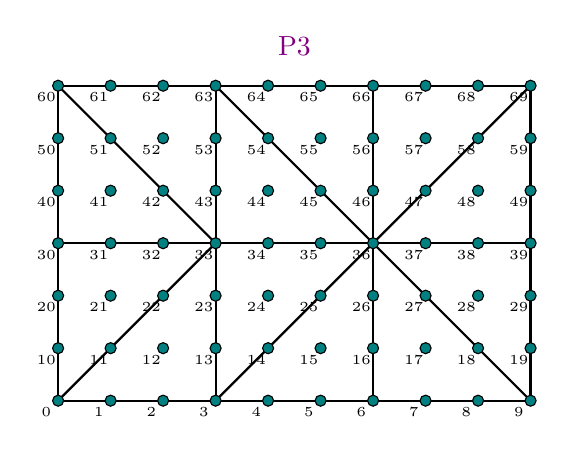
\begin{tikzpicture} 
\node[violet] at (3,4.5) {P3}; 
\draw[thick] (0,0) -- (6,0) -- (6,4) -- (0,4) -- cycle; 
\draw[thick] (0,2) -- (6,2) ; 
\draw[thick] (2,0) -- (2,4) ; 
\draw[thick] (4,0) -- (4,4) ; 
\draw[thick] (0,0) -- (2,2) -- (0,4) ; 
\draw[thick] (2,0) -- (4,2) -- (2,4) ; 
\draw[thick] (6,0) -- (4,2) -- (6,4) ; 
\draw[black,fill=teal] ( 0.000000 , 0.000000)     circle (2pt); 
\node[] at ( -0.150000, -0.150000 ) {\tiny 0 }; 
\draw[black,fill=teal] ( 0.666667 , 0.000000)     circle (2pt); 
\node[] at ( 0.516667, -0.150000 ) {\tiny 1 }; 
\draw[black,fill=teal] ( 1.333333 , 0.000000)     circle (2pt); 
\node[] at ( 1.183333, -0.150000 ) {\tiny 2 }; 
\draw[black,fill=teal] ( 2.000000 , 0.000000)     circle (2pt); 
\node[] at ( 1.850000, -0.150000 ) {\tiny 3 }; 
\draw[black,fill=teal] ( 2.666667 , 0.000000)     circle (2pt); 
\node[] at ( 2.516667, -0.150000 ) {\tiny 4 }; 
\draw[black,fill=teal] ( 3.333333 , 0.000000)     circle (2pt); 
\node[] at ( 3.183333, -0.150000 ) {\tiny 5 }; 
\draw[black,fill=teal] ( 4.000000 , 0.000000)     circle (2pt); 
\node[] at ( 3.850000, -0.150000 ) {\tiny 6 }; 
\draw[black,fill=teal] ( 4.666667 , 0.000000)     circle (2pt); 
\node[] at ( 4.516667, -0.150000 ) {\tiny 7 }; 
\draw[black,fill=teal] ( 5.333333 , 0.000000)     circle (2pt); 
\node[] at ( 5.183333, -0.150000 ) {\tiny 8 }; 
\draw[black,fill=teal] ( 6.000000 , 0.000000)     circle (2pt); 
\node[] at ( 5.850000, -0.150000 ) {\tiny 9 }; 
\draw[black,fill=teal] ( 0.000000 , 0.666667)     circle (2pt); 
\node[] at ( -0.150000, 0.516667 ) {\tiny 10 }; 
\draw[black,fill=teal] ( 0.666667 , 0.666667)     circle (2pt); 
\node[] at ( 0.516667, 0.516667 ) {\tiny 11 }; 
\draw[black,fill=teal] ( 1.333333 , 0.666667)     circle (2pt); 
\node[] at ( 1.183333, 0.516667 ) {\tiny 12 }; 
\draw[black,fill=teal] ( 2.000000 , 0.666667)     circle (2pt); 
\node[] at ( 1.850000, 0.516667 ) {\tiny 13 }; 
\draw[black,fill=teal] ( 2.666667 , 0.666667)     circle (2pt); 
\node[] at ( 2.516667, 0.516667 ) {\tiny 14 }; 
\draw[black,fill=teal] ( 3.333333 , 0.666667)     circle (2pt); 
\node[] at ( 3.183333, 0.516667 ) {\tiny 15 }; 
\draw[black,fill=teal] ( 4.000000 , 0.666667)     circle (2pt); 
\node[] at ( 3.850000, 0.516667 ) {\tiny 16 }; 
\draw[black,fill=teal] ( 4.666667 , 0.666667)     circle (2pt); 
\node[] at ( 4.516667, 0.516667 ) {\tiny 17 }; 
\draw[black,fill=teal] ( 5.333333 , 0.666667)     circle (2pt); 
\node[] at ( 5.183333, 0.516667 ) {\tiny 18 }; 
\draw[black,fill=teal] ( 6.000000 , 0.666667)     circle (2pt); 
\node[] at ( 5.850000, 0.516667 ) {\tiny 19 }; 
\draw[black,fill=teal] ( 0.000000 , 1.333333)     circle (2pt); 
\node[] at ( -0.150000, 1.183333 ) {\tiny 20 }; 
\draw[black,fill=teal] ( 0.666667 , 1.333333)     circle (2pt); 
\node[] at ( 0.516667, 1.183333 ) {\tiny 21 }; 
\draw[black,fill=teal] ( 1.333333 , 1.333333)     circle (2pt); 
\node[] at ( 1.183333, 1.183333 ) {\tiny 22 }; 
\draw[black,fill=teal] ( 2.000000 , 1.333333)     circle (2pt); 
\node[] at ( 1.850000, 1.183333 ) {\tiny 23 }; 
\draw[black,fill=teal] ( 2.666667 , 1.333333)     circle (2pt); 
\node[] at ( 2.516667, 1.183333 ) {\tiny 24 }; 
\draw[black,fill=teal] ( 3.333333 , 1.333333)     circle (2pt); 
\node[] at ( 3.183333, 1.183333 ) {\tiny 25 }; 
\draw[black,fill=teal] ( 4.000000 , 1.333333)     circle (2pt); 
\node[] at ( 3.850000, 1.183333 ) {\tiny 26 }; 
\draw[black,fill=teal] ( 4.666667 , 1.333333)     circle (2pt); 
\node[] at ( 4.516667, 1.183333 ) {\tiny 27 }; 
\draw[black,fill=teal] ( 5.333333 , 1.333333)     circle (2pt); 
\node[] at ( 5.183333, 1.183333 ) {\tiny 28 }; 
\draw[black,fill=teal] ( 6.000000 , 1.333333)     circle (2pt); 
\node[] at ( 5.850000, 1.183333 ) {\tiny 29 }; 
\draw[black,fill=teal] ( 0.000000 , 2.000000)     circle (2pt); 
\node[] at ( -0.150000, 1.850000 ) {\tiny 30 }; 
\draw[black,fill=teal] ( 0.666667 , 2.000000)     circle (2pt); 
\node[] at ( 0.516667, 1.850000 ) {\tiny 31 }; 
\draw[black,fill=teal] ( 1.333333 , 2.000000)     circle (2pt); 
\node[] at ( 1.183333, 1.850000 ) {\tiny 32 }; 
\draw[black,fill=teal] ( 2.000000 , 2.000000)     circle (2pt); 
\node[] at ( 1.850000, 1.850000 ) {\tiny 33 }; 
\draw[black,fill=teal] ( 2.666667 , 2.000000)     circle (2pt); 
\node[] at ( 2.516667, 1.850000 ) {\tiny 34 }; 
\draw[black,fill=teal] ( 3.333333 , 2.000000)     circle (2pt); 
\node[] at ( 3.183333, 1.850000 ) {\tiny 35 }; 
\draw[black,fill=teal] ( 4.000000 , 2.000000)     circle (2pt); 
\node[] at ( 3.850000, 1.850000 ) {\tiny 36 }; 
\draw[black,fill=teal] ( 4.666667 , 2.000000)     circle (2pt); 
\node[] at ( 4.516667, 1.850000 ) {\tiny 37 }; 
\draw[black,fill=teal] ( 5.333333 , 2.000000)     circle (2pt); 
\node[] at ( 5.183333, 1.850000 ) {\tiny 38 }; 
\draw[black,fill=teal] ( 6.000000 , 2.000000)     circle (2pt); 
\node[] at ( 5.850000, 1.850000 ) {\tiny 39 }; 
\draw[black,fill=teal] ( 0.000000 , 2.666667)     circle (2pt); 
\node[] at ( -0.150000, 2.516667 ) {\tiny 40 }; 
\draw[black,fill=teal] ( 0.666667 , 2.666667)     circle (2pt); 
\node[] at ( 0.516667, 2.516667 ) {\tiny 41 }; 
\draw[black,fill=teal] ( 1.333333 , 2.666667)     circle (2pt); 
\node[] at ( 1.183333, 2.516667 ) {\tiny 42 }; 
\draw[black,fill=teal] ( 2.000000 , 2.666667)     circle (2pt); 
\node[] at ( 1.850000, 2.516667 ) {\tiny 43 }; 
\draw[black,fill=teal] ( 2.666667 , 2.666667)     circle (2pt); 
\node[] at ( 2.516667, 2.516667 ) {\tiny 44 }; 
\draw[black,fill=teal] ( 3.333333 , 2.666667)     circle (2pt); 
\node[] at ( 3.183333, 2.516667 ) {\tiny 45 }; 
\draw[black,fill=teal] ( 4.000000 , 2.666667)     circle (2pt); 
\node[] at ( 3.850000, 2.516667 ) {\tiny 46 }; 
\draw[black,fill=teal] ( 4.666667 , 2.666667)     circle (2pt); 
\node[] at ( 4.516667, 2.516667 ) {\tiny 47 }; 
\draw[black,fill=teal] ( 5.333333 , 2.666667)     circle (2pt); 
\node[] at ( 5.183333, 2.516667 ) {\tiny 48 }; 
\draw[black,fill=teal] ( 6.000000 , 2.666667)     circle (2pt); 
\node[] at ( 5.850000, 2.516667 ) {\tiny 49 }; 
\draw[black,fill=teal] ( 0.000000 , 3.333333)     circle (2pt); 
\node[] at ( -0.150000, 3.183333 ) {\tiny 50 }; 
\draw[black,fill=teal] ( 0.666667 , 3.333333)     circle (2pt); 
\node[] at ( 0.516667, 3.183333 ) {\tiny 51 }; 
\draw[black,fill=teal] ( 1.333333 , 3.333333)     circle (2pt); 
\node[] at ( 1.183333, 3.183333 ) {\tiny 52 }; 
\draw[black,fill=teal] ( 2.000000 , 3.333333)     circle (2pt); 
\node[] at ( 1.850000, 3.183333 ) {\tiny 53 }; 
\draw[black,fill=teal] ( 2.666667 , 3.333333)     circle (2pt); 
\node[] at ( 2.516667, 3.183333 ) {\tiny 54 }; 
\draw[black,fill=teal] ( 3.333333 , 3.333333)     circle (2pt); 
\node[] at ( 3.183333, 3.183333 ) {\tiny 55 }; 
\draw[black,fill=teal] ( 4.000000 , 3.333333)     circle (2pt); 
\node[] at ( 3.850000, 3.183333 ) {\tiny 56 }; 
\draw[black,fill=teal] ( 4.666667 , 3.333333)     circle (2pt); 
\node[] at ( 4.516667, 3.183333 ) {\tiny 57 }; 
\draw[black,fill=teal] ( 5.333333 , 3.333333)     circle (2pt); 
\node[] at ( 5.183333, 3.183333 ) {\tiny 58 }; 
\draw[black,fill=teal] ( 6.000000 , 3.333333)     circle (2pt); 
\node[] at ( 5.850000, 3.183333 ) {\tiny 59 }; 
\draw[black,fill=teal] ( 0.000000 , 4.000000)     circle (2pt); 
\node[] at ( -0.150000, 3.850000 ) {\tiny 60 }; 
\draw[black,fill=teal] ( 0.666667 , 4.000000)     circle (2pt); 
\node[] at ( 0.516667, 3.850000 ) {\tiny 61 }; 
\draw[black,fill=teal] ( 1.333333 , 4.000000)     circle (2pt); 
\node[] at ( 1.183333, 3.850000 ) {\tiny 62 }; 
\draw[black,fill=teal] ( 2.000000 , 4.000000)     circle (2pt); 
\node[] at ( 1.850000, 3.850000 ) {\tiny 63 }; 
\draw[black,fill=teal] ( 2.666667 , 4.000000)     circle (2pt); 
\node[] at ( 2.516667, 3.850000 ) {\tiny 64 }; 
\draw[black,fill=teal] ( 3.333333 , 4.000000)     circle (2pt); 
\node[] at ( 3.183333, 3.850000 ) {\tiny 65 }; 
\draw[black,fill=teal] ( 4.000000 , 4.000000)     circle (2pt); 
\node[] at ( 3.850000, 3.850000 ) {\tiny 66 }; 
\draw[black,fill=teal] ( 4.666667 , 4.000000)     circle (2pt); 
\node[] at ( 4.516667, 3.850000 ) {\tiny 67 }; 
\draw[black,fill=teal] ( 5.333333 , 4.000000)     circle (2pt); 
\node[] at ( 5.183333, 3.850000 ) {\tiny 68 }; 
\draw[black,fill=teal] ( 6.000000 , 4.000000)     circle (2pt); 
\node[] at ( 5.850000, 3.850000 ) {\tiny 69 }; 
\end{tikzpicture} 
\end{center} 


\begin{tiny}
\verbatiminput{iconV_P3.ascii}
\end{tiny}

%--------------------------------
\newpage
\begin{center} 
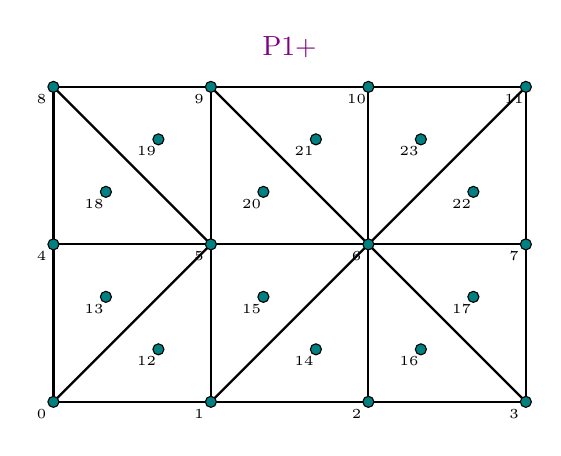
\begin{tikzpicture} 
\node[violet] at (3,4.5) {P1+}; 
\draw[thick] (0,0) -- (6,0) -- (6,4) -- (0,4) -- cycle; 
\draw[thick] (0,2) -- (6,2) ; 
\draw[thick] (2,0) -- (2,4) ; 
\draw[thick] (4,0) -- (4,4) ; 
\draw[thick] (0,0) -- (2,2) -- (0,4) ; 
\draw[thick] (2,0) -- (4,2) -- (2,4) ; 
\draw[thick] (6,0) -- (4,2) -- (6,4) ; 
\draw[black,fill=teal] ( 0.000000 , 0.000000)     circle (2pt); 
\node[] at ( -0.150000, -0.150000 ) {\tiny 0 }; 
\draw[black,fill=teal] ( 2.000000 , 0.000000)     circle (2pt); 
\node[] at ( 1.850000, -0.150000 ) {\tiny 1 }; 
\draw[black,fill=teal] ( 4.000000 , 0.000000)     circle (2pt); 
\node[] at ( 3.850000, -0.150000 ) {\tiny 2 }; 
\draw[black,fill=teal] ( 6.000000 , 0.000000)     circle (2pt); 
\node[] at ( 5.850000, -0.150000 ) {\tiny 3 }; 
\draw[black,fill=teal] ( 0.000000 , 2.000000)     circle (2pt); 
\node[] at ( -0.150000, 1.850000 ) {\tiny 4 }; 
\draw[black,fill=teal] ( 2.000000 , 2.000000)     circle (2pt); 
\node[] at ( 1.850000, 1.850000 ) {\tiny 5 }; 
\draw[black,fill=teal] ( 4.000000 , 2.000000)     circle (2pt); 
\node[] at ( 3.850000, 1.850000 ) {\tiny 6 }; 
\draw[black,fill=teal] ( 6.000000 , 2.000000)     circle (2pt); 
\node[] at ( 5.850000, 1.850000 ) {\tiny 7 }; 
\draw[black,fill=teal] ( 0.000000 , 4.000000)     circle (2pt); 
\node[] at ( -0.150000, 3.850000 ) {\tiny 8 }; 
\draw[black,fill=teal] ( 2.000000 , 4.000000)     circle (2pt); 
\node[] at ( 1.850000, 3.850000 ) {\tiny 9 }; 
\draw[black,fill=teal] ( 4.000000 , 4.000000)     circle (2pt); 
\node[] at ( 3.850000, 3.850000 ) {\tiny 10 }; 
\draw[black,fill=teal] ( 6.000000 , 4.000000)     circle (2pt); 
\node[] at ( 5.850000, 3.850000 ) {\tiny 11 }; 
\draw[black,fill=teal] ( 1.333333 , 0.666667)     circle (2pt); 
\node[] at ( 1.183333, 0.516667 ) {\tiny 12 }; 
\draw[black,fill=teal] ( 0.666667 , 1.333333)     circle (2pt); 
\node[] at ( 0.516667, 1.183333 ) {\tiny 13 }; 
\draw[black,fill=teal] ( 3.333333 , 0.666667)     circle (2pt); 
\node[] at ( 3.183333, 0.516667 ) {\tiny 14 }; 
\draw[black,fill=teal] ( 2.666667 , 1.333333)     circle (2pt); 
\node[] at ( 2.516667, 1.183333 ) {\tiny 15 }; 
\draw[black,fill=teal] ( 4.666667 , 0.666667)     circle (2pt); 
\node[] at ( 4.516667, 0.516667 ) {\tiny 16 }; 
\draw[black,fill=teal] ( 5.333333 , 1.333333)     circle (2pt); 
\node[] at ( 5.183333, 1.183333 ) {\tiny 17 }; 
\draw[black,fill=teal] ( 0.666667 , 2.666667)     circle (2pt); 
\node[] at ( 0.516667, 2.516667 ) {\tiny 18 }; 
\draw[black,fill=teal] ( 1.333333 , 3.333333)     circle (2pt); 
\node[] at ( 1.183333, 3.183333 ) {\tiny 19 }; 
\draw[black,fill=teal] ( 2.666667 , 2.666667)     circle (2pt); 
\node[] at ( 2.516667, 2.516667 ) {\tiny 20 }; 
\draw[black,fill=teal] ( 3.333333 , 3.333333)     circle (2pt); 
\node[] at ( 3.183333, 3.183333 ) {\tiny 21 }; 
\draw[black,fill=teal] ( 5.333333 , 2.666667)     circle (2pt); 
\node[] at ( 5.183333, 2.516667 ) {\tiny 22 }; 
\draw[black,fill=teal] ( 4.666667 , 3.333333)     circle (2pt); 
\node[] at ( 4.516667, 3.183333 ) {\tiny 23 }; 
\end{tikzpicture} 
\end{center} 


\begin{tiny}
\verbatiminput{iconV_P1+.ascii}
\end{tiny}

%--------------------------------
\newpage
\begin{center} 
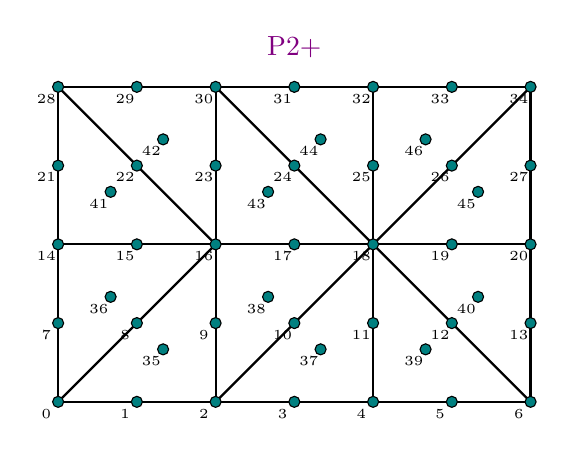
\begin{tikzpicture} 
\node[violet] at (3,4.5) {P2+}; 
\draw[thick] (0,0) -- (6,0) -- (6,4) -- (0,4) -- cycle; 
\draw[thick] (0,2) -- (6,2) ; 
\draw[thick] (2,0) -- (2,4) ; 
\draw[thick] (4,0) -- (4,4) ; 
\draw[thick] (0,0) -- (2,2) -- (0,4) ; 
\draw[thick] (2,0) -- (4,2) -- (2,4) ; 
\draw[thick] (6,0) -- (4,2) -- (6,4) ; 
\draw[black,fill=teal] ( 0.000000 , 0.000000)     circle (2pt); 
\node[] at ( -0.150000, -0.150000 ) {\tiny 0 }; 
\draw[black,fill=teal] ( 1.000000 , 0.000000)     circle (2pt); 
\node[] at ( 0.850000, -0.150000 ) {\tiny 1 }; 
\draw[black,fill=teal] ( 2.000000 , 0.000000)     circle (2pt); 
\node[] at ( 1.850000, -0.150000 ) {\tiny 2 }; 
\draw[black,fill=teal] ( 3.000000 , 0.000000)     circle (2pt); 
\node[] at ( 2.850000, -0.150000 ) {\tiny 3 }; 
\draw[black,fill=teal] ( 4.000000 , 0.000000)     circle (2pt); 
\node[] at ( 3.850000, -0.150000 ) {\tiny 4 }; 
\draw[black,fill=teal] ( 5.000000 , 0.000000)     circle (2pt); 
\node[] at ( 4.850000, -0.150000 ) {\tiny 5 }; 
\draw[black,fill=teal] ( 6.000000 , 0.000000)     circle (2pt); 
\node[] at ( 5.850000, -0.150000 ) {\tiny 6 }; 
\draw[black,fill=teal] ( 0.000000 , 1.000000)     circle (2pt); 
\node[] at ( -0.150000, 0.850000 ) {\tiny 7 }; 
\draw[black,fill=teal] ( 1.000000 , 1.000000)     circle (2pt); 
\node[] at ( 0.850000, 0.850000 ) {\tiny 8 }; 
\draw[black,fill=teal] ( 2.000000 , 1.000000)     circle (2pt); 
\node[] at ( 1.850000, 0.850000 ) {\tiny 9 }; 
\draw[black,fill=teal] ( 3.000000 , 1.000000)     circle (2pt); 
\node[] at ( 2.850000, 0.850000 ) {\tiny 10 }; 
\draw[black,fill=teal] ( 4.000000 , 1.000000)     circle (2pt); 
\node[] at ( 3.850000, 0.850000 ) {\tiny 11 }; 
\draw[black,fill=teal] ( 5.000000 , 1.000000)     circle (2pt); 
\node[] at ( 4.850000, 0.850000 ) {\tiny 12 }; 
\draw[black,fill=teal] ( 6.000000 , 1.000000)     circle (2pt); 
\node[] at ( 5.850000, 0.850000 ) {\tiny 13 }; 
\draw[black,fill=teal] ( 0.000000 , 2.000000)     circle (2pt); 
\node[] at ( -0.150000, 1.850000 ) {\tiny 14 }; 
\draw[black,fill=teal] ( 1.000000 , 2.000000)     circle (2pt); 
\node[] at ( 0.850000, 1.850000 ) {\tiny 15 }; 
\draw[black,fill=teal] ( 2.000000 , 2.000000)     circle (2pt); 
\node[] at ( 1.850000, 1.850000 ) {\tiny 16 }; 
\draw[black,fill=teal] ( 3.000000 , 2.000000)     circle (2pt); 
\node[] at ( 2.850000, 1.850000 ) {\tiny 17 }; 
\draw[black,fill=teal] ( 4.000000 , 2.000000)     circle (2pt); 
\node[] at ( 3.850000, 1.850000 ) {\tiny 18 }; 
\draw[black,fill=teal] ( 5.000000 , 2.000000)     circle (2pt); 
\node[] at ( 4.850000, 1.850000 ) {\tiny 19 }; 
\draw[black,fill=teal] ( 6.000000 , 2.000000)     circle (2pt); 
\node[] at ( 5.850000, 1.850000 ) {\tiny 20 }; 
\draw[black,fill=teal] ( 0.000000 , 3.000000)     circle (2pt); 
\node[] at ( -0.150000, 2.850000 ) {\tiny 21 }; 
\draw[black,fill=teal] ( 1.000000 , 3.000000)     circle (2pt); 
\node[] at ( 0.850000, 2.850000 ) {\tiny 22 }; 
\draw[black,fill=teal] ( 2.000000 , 3.000000)     circle (2pt); 
\node[] at ( 1.850000, 2.850000 ) {\tiny 23 }; 
\draw[black,fill=teal] ( 3.000000 , 3.000000)     circle (2pt); 
\node[] at ( 2.850000, 2.850000 ) {\tiny 24 }; 
\draw[black,fill=teal] ( 4.000000 , 3.000000)     circle (2pt); 
\node[] at ( 3.850000, 2.850000 ) {\tiny 25 }; 
\draw[black,fill=teal] ( 5.000000 , 3.000000)     circle (2pt); 
\node[] at ( 4.850000, 2.850000 ) {\tiny 26 }; 
\draw[black,fill=teal] ( 6.000000 , 3.000000)     circle (2pt); 
\node[] at ( 5.850000, 2.850000 ) {\tiny 27 }; 
\draw[black,fill=teal] ( 0.000000 , 4.000000)     circle (2pt); 
\node[] at ( -0.150000, 3.850000 ) {\tiny 28 }; 
\draw[black,fill=teal] ( 1.000000 , 4.000000)     circle (2pt); 
\node[] at ( 0.850000, 3.850000 ) {\tiny 29 }; 
\draw[black,fill=teal] ( 2.000000 , 4.000000)     circle (2pt); 
\node[] at ( 1.850000, 3.850000 ) {\tiny 30 }; 
\draw[black,fill=teal] ( 3.000000 , 4.000000)     circle (2pt); 
\node[] at ( 2.850000, 3.850000 ) {\tiny 31 }; 
\draw[black,fill=teal] ( 4.000000 , 4.000000)     circle (2pt); 
\node[] at ( 3.850000, 3.850000 ) {\tiny 32 }; 
\draw[black,fill=teal] ( 5.000000 , 4.000000)     circle (2pt); 
\node[] at ( 4.850000, 3.850000 ) {\tiny 33 }; 
\draw[black,fill=teal] ( 6.000000 , 4.000000)     circle (2pt); 
\node[] at ( 5.850000, 3.850000 ) {\tiny 34 }; 
\draw[black,fill=teal] ( 1.333333 , 0.666667)     circle (2pt); 
\node[] at ( 1.183333, 0.516667 ) {\tiny 35 }; 
\draw[black,fill=teal] ( 0.666667 , 1.333333)     circle (2pt); 
\node[] at ( 0.516667, 1.183333 ) {\tiny 36 }; 
\draw[black,fill=teal] ( 3.333333 , 0.666667)     circle (2pt); 
\node[] at ( 3.183333, 0.516667 ) {\tiny 37 }; 
\draw[black,fill=teal] ( 2.666667 , 1.333333)     circle (2pt); 
\node[] at ( 2.516667, 1.183333 ) {\tiny 38 }; 
\draw[black,fill=teal] ( 4.666667 , 0.666667)     circle (2pt); 
\node[] at ( 4.516667, 0.516667 ) {\tiny 39 }; 
\draw[black,fill=teal] ( 5.333333 , 1.333333)     circle (2pt); 
\node[] at ( 5.183333, 1.183333 ) {\tiny 40 }; 
\draw[black,fill=teal] ( 0.666667 , 2.666667)     circle (2pt); 
\node[] at ( 0.516667, 2.516667 ) {\tiny 41 }; 
\draw[black,fill=teal] ( 1.333333 , 3.333333)     circle (2pt); 
\node[] at ( 1.183333, 3.183333 ) {\tiny 42 }; 
\draw[black,fill=teal] ( 2.666667 , 2.666667)     circle (2pt); 
\node[] at ( 2.516667, 2.516667 ) {\tiny 43 }; 
\draw[black,fill=teal] ( 3.333333 , 3.333333)     circle (2pt); 
\node[] at ( 3.183333, 3.183333 ) {\tiny 44 }; 
\draw[black,fill=teal] ( 5.333333 , 2.666667)     circle (2pt); 
\node[] at ( 5.183333, 2.516667 ) {\tiny 45 }; 
\draw[black,fill=teal] ( 4.666667 , 3.333333)     circle (2pt); 
\node[] at ( 4.516667, 3.183333 ) {\tiny 46 }; 
\end{tikzpicture} 
\end{center} 


\begin{tiny}
\verbatiminput{iconV_P2+.ascii}
\end{tiny}

%--------------------------------
\newpage
\begin{center} 
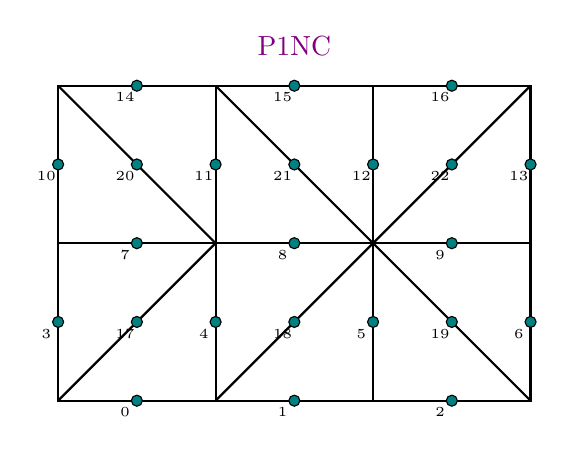
\begin{tikzpicture} 
\node[violet] at (3,4.5) {P1NC}; 
\draw[thick] (0,0) -- (6,0) -- (6,4) -- (0,4) -- cycle; 
\draw[thick] (0,2) -- (6,2) ; 
\draw[thick] (2,0) -- (2,4) ; 
\draw[thick] (4,0) -- (4,4) ; 
\draw[thick] (0,0) -- (2,2) -- (0,4) ; 
\draw[thick] (2,0) -- (4,2) -- (2,4) ; 
\draw[thick] (6,0) -- (4,2) -- (6,4) ; 
\draw[black,fill=teal] ( 1.000000 , 0.000000)     circle (2pt); 
\node[] at ( 0.850000, -0.150000 ) {\tiny 0 }; 
\draw[black,fill=teal] ( 3.000000 , 0.000000)     circle (2pt); 
\node[] at ( 2.850000, -0.150000 ) {\tiny 1 }; 
\draw[black,fill=teal] ( 5.000000 , 0.000000)     circle (2pt); 
\node[] at ( 4.850000, -0.150000 ) {\tiny 2 }; 
\draw[black,fill=teal] ( 0.000000 , 1.000000)     circle (2pt); 
\node[] at ( -0.150000, 0.850000 ) {\tiny 3 }; 
\draw[black,fill=teal] ( 2.000000 , 1.000000)     circle (2pt); 
\node[] at ( 1.850000, 0.850000 ) {\tiny 4 }; 
\draw[black,fill=teal] ( 4.000000 , 1.000000)     circle (2pt); 
\node[] at ( 3.850000, 0.850000 ) {\tiny 5 }; 
\draw[black,fill=teal] ( 6.000000 , 1.000000)     circle (2pt); 
\node[] at ( 5.850000, 0.850000 ) {\tiny 6 }; 
\draw[black,fill=teal] ( 1.000000 , 2.000000)     circle (2pt); 
\node[] at ( 0.850000, 1.850000 ) {\tiny 7 }; 
\draw[black,fill=teal] ( 3.000000 , 2.000000)     circle (2pt); 
\node[] at ( 2.850000, 1.850000 ) {\tiny 8 }; 
\draw[black,fill=teal] ( 5.000000 , 2.000000)     circle (2pt); 
\node[] at ( 4.850000, 1.850000 ) {\tiny 9 }; 
\draw[black,fill=teal] ( 0.000000 , 3.000000)     circle (2pt); 
\node[] at ( -0.150000, 2.850000 ) {\tiny 10 }; 
\draw[black,fill=teal] ( 2.000000 , 3.000000)     circle (2pt); 
\node[] at ( 1.850000, 2.850000 ) {\tiny 11 }; 
\draw[black,fill=teal] ( 4.000000 , 3.000000)     circle (2pt); 
\node[] at ( 3.850000, 2.850000 ) {\tiny 12 }; 
\draw[black,fill=teal] ( 6.000000 , 3.000000)     circle (2pt); 
\node[] at ( 5.850000, 2.850000 ) {\tiny 13 }; 
\draw[black,fill=teal] ( 1.000000 , 4.000000)     circle (2pt); 
\node[] at ( 0.850000, 3.850000 ) {\tiny 14 }; 
\draw[black,fill=teal] ( 3.000000 , 4.000000)     circle (2pt); 
\node[] at ( 2.850000, 3.850000 ) {\tiny 15 }; 
\draw[black,fill=teal] ( 5.000000 , 4.000000)     circle (2pt); 
\node[] at ( 4.850000, 3.850000 ) {\tiny 16 }; 
\draw[black,fill=teal] ( 1.000000 , 1.000000)     circle (2pt); 
\node[] at ( 0.850000, 0.850000 ) {\tiny 17 }; 
\draw[black,fill=teal] ( 3.000000 , 1.000000)     circle (2pt); 
\node[] at ( 2.850000, 0.850000 ) {\tiny 18 }; 
\draw[black,fill=teal] ( 5.000000 , 1.000000)     circle (2pt); 
\node[] at ( 4.850000, 0.850000 ) {\tiny 19 }; 
\draw[black,fill=teal] ( 1.000000 , 3.000000)     circle (2pt); 
\node[] at ( 0.850000, 2.850000 ) {\tiny 20 }; 
\draw[black,fill=teal] ( 3.000000 , 3.000000)     circle (2pt); 
\node[] at ( 2.850000, 2.850000 ) {\tiny 21 }; 
\draw[black,fill=teal] ( 5.000000 , 3.000000)     circle (2pt); 
\node[] at ( 4.850000, 2.850000 ) {\tiny 22 }; 
\end{tikzpicture} 
\end{center} 


\begin{tiny}
\verbatiminput{iconV_P1NC.ascii}
\end{tiny}

%--------------------------------
\newpage
\begin{center} 
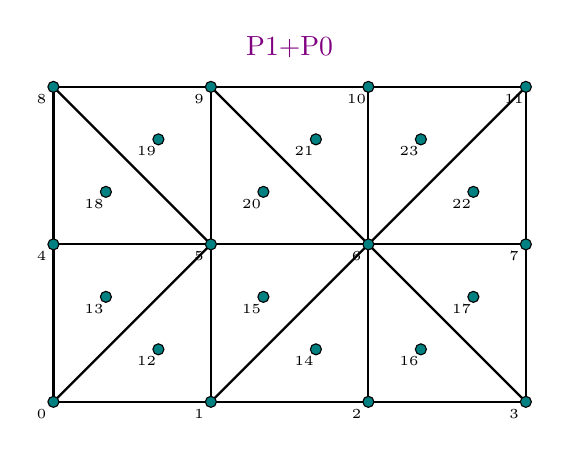
\begin{tikzpicture} 
\node[violet] at (3,4.5) {P1+P0}; 
\draw[thick] (0,0) -- (6,0) -- (6,4) -- (0,4) -- cycle; 
\draw[thick] (0,2) -- (6,2) ; 
\draw[thick] (2,0) -- (2,4) ; 
\draw[thick] (4,0) -- (4,4) ; 
\draw[thick] (0,0) -- (2,2) -- (0,4) ; 
\draw[thick] (2,0) -- (4,2) -- (2,4) ; 
\draw[thick] (6,0) -- (4,2) -- (6,4) ; 
\draw[black,fill=teal] ( 0.000000 , 0.000000)     circle (2pt); 
\node[] at ( -0.150000, -0.150000 ) {\tiny 0 }; 
\draw[black,fill=teal] ( 2.000000 , 0.000000)     circle (2pt); 
\node[] at ( 1.850000, -0.150000 ) {\tiny 1 }; 
\draw[black,fill=teal] ( 4.000000 , 0.000000)     circle (2pt); 
\node[] at ( 3.850000, -0.150000 ) {\tiny 2 }; 
\draw[black,fill=teal] ( 6.000000 , 0.000000)     circle (2pt); 
\node[] at ( 5.850000, -0.150000 ) {\tiny 3 }; 
\draw[black,fill=teal] ( 0.000000 , 2.000000)     circle (2pt); 
\node[] at ( -0.150000, 1.850000 ) {\tiny 4 }; 
\draw[black,fill=teal] ( 2.000000 , 2.000000)     circle (2pt); 
\node[] at ( 1.850000, 1.850000 ) {\tiny 5 }; 
\draw[black,fill=teal] ( 4.000000 , 2.000000)     circle (2pt); 
\node[] at ( 3.850000, 1.850000 ) {\tiny 6 }; 
\draw[black,fill=teal] ( 6.000000 , 2.000000)     circle (2pt); 
\node[] at ( 5.850000, 1.850000 ) {\tiny 7 }; 
\draw[black,fill=teal] ( 0.000000 , 4.000000)     circle (2pt); 
\node[] at ( -0.150000, 3.850000 ) {\tiny 8 }; 
\draw[black,fill=teal] ( 2.000000 , 4.000000)     circle (2pt); 
\node[] at ( 1.850000, 3.850000 ) {\tiny 9 }; 
\draw[black,fill=teal] ( 4.000000 , 4.000000)     circle (2pt); 
\node[] at ( 3.850000, 3.850000 ) {\tiny 10 }; 
\draw[black,fill=teal] ( 6.000000 , 4.000000)     circle (2pt); 
\node[] at ( 5.850000, 3.850000 ) {\tiny 11 }; 
\draw[black,fill=teal] ( 1.333333 , 0.666667)     circle (2pt); 
\node[] at ( 1.183333, 0.516667 ) {\tiny 12 }; 
\draw[black,fill=teal] ( 0.666667 , 1.333333)     circle (2pt); 
\node[] at ( 0.516667, 1.183333 ) {\tiny 13 }; 
\draw[black,fill=teal] ( 3.333333 , 0.666667)     circle (2pt); 
\node[] at ( 3.183333, 0.516667 ) {\tiny 14 }; 
\draw[black,fill=teal] ( 2.666667 , 1.333333)     circle (2pt); 
\node[] at ( 2.516667, 1.183333 ) {\tiny 15 }; 
\draw[black,fill=teal] ( 4.666667 , 0.666667)     circle (2pt); 
\node[] at ( 4.516667, 0.516667 ) {\tiny 16 }; 
\draw[black,fill=teal] ( 5.333333 , 1.333333)     circle (2pt); 
\node[] at ( 5.183333, 1.183333 ) {\tiny 17 }; 
\draw[black,fill=teal] ( 0.666667 , 2.666667)     circle (2pt); 
\node[] at ( 0.516667, 2.516667 ) {\tiny 18 }; 
\draw[black,fill=teal] ( 1.333333 , 3.333333)     circle (2pt); 
\node[] at ( 1.183333, 3.183333 ) {\tiny 19 }; 
\draw[black,fill=teal] ( 2.666667 , 2.666667)     circle (2pt); 
\node[] at ( 2.516667, 2.516667 ) {\tiny 20 }; 
\draw[black,fill=teal] ( 3.333333 , 3.333333)     circle (2pt); 
\node[] at ( 3.183333, 3.183333 ) {\tiny 21 }; 
\draw[black,fill=teal] ( 5.333333 , 2.666667)     circle (2pt); 
\node[] at ( 5.183333, 2.516667 ) {\tiny 22 }; 
\draw[black,fill=teal] ( 4.666667 , 3.333333)     circle (2pt); 
\node[] at ( 4.516667, 3.183333 ) {\tiny 23 }; 
\end{tikzpicture} 
\end{center} 


\begin{tiny}
\verbatiminput{iconV_P1+P0.ascii}
\end{tiny}

%--------------------------------
\newpage
\begin{center} 
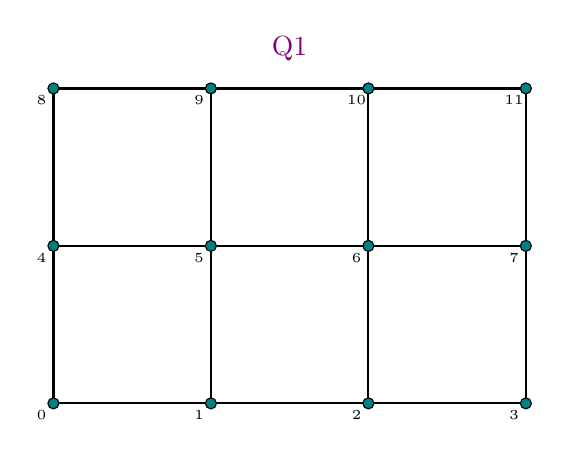
\begin{tikzpicture} 
\node[violet] at (3,4.5) {Q1}; 
\draw[thick] (0,0) -- (6,0) -- (6,4) -- (0,4) -- cycle; 
\draw[thick] (0,2) -- (6,2) ; 
\draw[thick] (2,0) -- (2,4) ; 
\draw[thick] (4,0) -- (4,4) ; 
\draw[black,fill=teal] ( 0.000000 , 0.000000)     circle (2pt); 
\node[] at ( -0.150000, -0.150000 ) {\tiny 0 }; 
\draw[black,fill=teal] ( 2.000000 , 0.000000)     circle (2pt); 
\node[] at ( 1.850000, -0.150000 ) {\tiny 1 }; 
\draw[black,fill=teal] ( 4.000000 , 0.000000)     circle (2pt); 
\node[] at ( 3.850000, -0.150000 ) {\tiny 2 }; 
\draw[black,fill=teal] ( 6.000000 , 0.000000)     circle (2pt); 
\node[] at ( 5.850000, -0.150000 ) {\tiny 3 }; 
\draw[black,fill=teal] ( 0.000000 , 2.000000)     circle (2pt); 
\node[] at ( -0.150000, 1.850000 ) {\tiny 4 }; 
\draw[black,fill=teal] ( 2.000000 , 2.000000)     circle (2pt); 
\node[] at ( 1.850000, 1.850000 ) {\tiny 5 }; 
\draw[black,fill=teal] ( 4.000000 , 2.000000)     circle (2pt); 
\node[] at ( 3.850000, 1.850000 ) {\tiny 6 }; 
\draw[black,fill=teal] ( 6.000000 , 2.000000)     circle (2pt); 
\node[] at ( 5.850000, 1.850000 ) {\tiny 7 }; 
\draw[black,fill=teal] ( 0.000000 , 4.000000)     circle (2pt); 
\node[] at ( -0.150000, 3.850000 ) {\tiny 8 }; 
\draw[black,fill=teal] ( 2.000000 , 4.000000)     circle (2pt); 
\node[] at ( 1.850000, 3.850000 ) {\tiny 9 }; 
\draw[black,fill=teal] ( 4.000000 , 4.000000)     circle (2pt); 
\node[] at ( 3.850000, 3.850000 ) {\tiny 10 }; 
\draw[black,fill=teal] ( 6.000000 , 4.000000)     circle (2pt); 
\node[] at ( 5.850000, 3.850000 ) {\tiny 11 }; 
\end{tikzpicture} 
\end{center} 


%--------------------------------
\begin{center} 
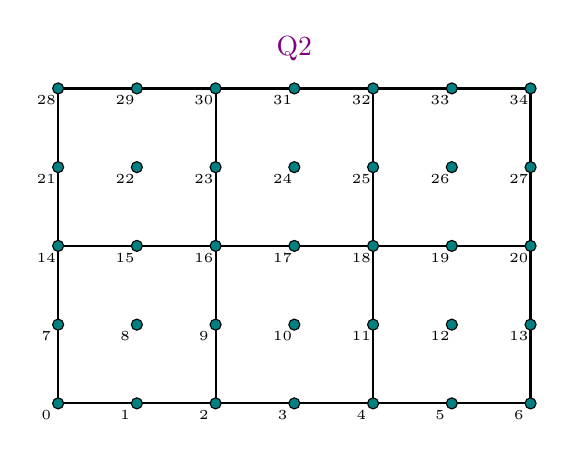
\begin{tikzpicture} 
\node[violet] at (3,4.5) {Q2}; 
\draw[thick] (0,0) -- (6,0) -- (6,4) -- (0,4) -- cycle; 
\draw[thick] (0,2) -- (6,2) ; 
\draw[thick] (2,0) -- (2,4) ; 
\draw[thick] (4,0) -- (4,4) ; 
\draw[black,fill=teal] ( 0.000000 , 0.000000)     circle (2pt); 
\node[] at ( -0.150000, -0.150000 ) {\tiny 0 }; 
\draw[black,fill=teal] ( 1.000000 , 0.000000)     circle (2pt); 
\node[] at ( 0.850000, -0.150000 ) {\tiny 1 }; 
\draw[black,fill=teal] ( 2.000000 , 0.000000)     circle (2pt); 
\node[] at ( 1.850000, -0.150000 ) {\tiny 2 }; 
\draw[black,fill=teal] ( 3.000000 , 0.000000)     circle (2pt); 
\node[] at ( 2.850000, -0.150000 ) {\tiny 3 }; 
\draw[black,fill=teal] ( 4.000000 , 0.000000)     circle (2pt); 
\node[] at ( 3.850000, -0.150000 ) {\tiny 4 }; 
\draw[black,fill=teal] ( 5.000000 , 0.000000)     circle (2pt); 
\node[] at ( 4.850000, -0.150000 ) {\tiny 5 }; 
\draw[black,fill=teal] ( 6.000000 , 0.000000)     circle (2pt); 
\node[] at ( 5.850000, -0.150000 ) {\tiny 6 }; 
\draw[black,fill=teal] ( 0.000000 , 1.000000)     circle (2pt); 
\node[] at ( -0.150000, 0.850000 ) {\tiny 7 }; 
\draw[black,fill=teal] ( 1.000000 , 1.000000)     circle (2pt); 
\node[] at ( 0.850000, 0.850000 ) {\tiny 8 }; 
\draw[black,fill=teal] ( 2.000000 , 1.000000)     circle (2pt); 
\node[] at ( 1.850000, 0.850000 ) {\tiny 9 }; 
\draw[black,fill=teal] ( 3.000000 , 1.000000)     circle (2pt); 
\node[] at ( 2.850000, 0.850000 ) {\tiny 10 }; 
\draw[black,fill=teal] ( 4.000000 , 1.000000)     circle (2pt); 
\node[] at ( 3.850000, 0.850000 ) {\tiny 11 }; 
\draw[black,fill=teal] ( 5.000000 , 1.000000)     circle (2pt); 
\node[] at ( 4.850000, 0.850000 ) {\tiny 12 }; 
\draw[black,fill=teal] ( 6.000000 , 1.000000)     circle (2pt); 
\node[] at ( 5.850000, 0.850000 ) {\tiny 13 }; 
\draw[black,fill=teal] ( 0.000000 , 2.000000)     circle (2pt); 
\node[] at ( -0.150000, 1.850000 ) {\tiny 14 }; 
\draw[black,fill=teal] ( 1.000000 , 2.000000)     circle (2pt); 
\node[] at ( 0.850000, 1.850000 ) {\tiny 15 }; 
\draw[black,fill=teal] ( 2.000000 , 2.000000)     circle (2pt); 
\node[] at ( 1.850000, 1.850000 ) {\tiny 16 }; 
\draw[black,fill=teal] ( 3.000000 , 2.000000)     circle (2pt); 
\node[] at ( 2.850000, 1.850000 ) {\tiny 17 }; 
\draw[black,fill=teal] ( 4.000000 , 2.000000)     circle (2pt); 
\node[] at ( 3.850000, 1.850000 ) {\tiny 18 }; 
\draw[black,fill=teal] ( 5.000000 , 2.000000)     circle (2pt); 
\node[] at ( 4.850000, 1.850000 ) {\tiny 19 }; 
\draw[black,fill=teal] ( 6.000000 , 2.000000)     circle (2pt); 
\node[] at ( 5.850000, 1.850000 ) {\tiny 20 }; 
\draw[black,fill=teal] ( 0.000000 , 3.000000)     circle (2pt); 
\node[] at ( -0.150000, 2.850000 ) {\tiny 21 }; 
\draw[black,fill=teal] ( 1.000000 , 3.000000)     circle (2pt); 
\node[] at ( 0.850000, 2.850000 ) {\tiny 22 }; 
\draw[black,fill=teal] ( 2.000000 , 3.000000)     circle (2pt); 
\node[] at ( 1.850000, 2.850000 ) {\tiny 23 }; 
\draw[black,fill=teal] ( 3.000000 , 3.000000)     circle (2pt); 
\node[] at ( 2.850000, 2.850000 ) {\tiny 24 }; 
\draw[black,fill=teal] ( 4.000000 , 3.000000)     circle (2pt); 
\node[] at ( 3.850000, 2.850000 ) {\tiny 25 }; 
\draw[black,fill=teal] ( 5.000000 , 3.000000)     circle (2pt); 
\node[] at ( 4.850000, 2.850000 ) {\tiny 26 }; 
\draw[black,fill=teal] ( 6.000000 , 3.000000)     circle (2pt); 
\node[] at ( 5.850000, 2.850000 ) {\tiny 27 }; 
\draw[black,fill=teal] ( 0.000000 , 4.000000)     circle (2pt); 
\node[] at ( -0.150000, 3.850000 ) {\tiny 28 }; 
\draw[black,fill=teal] ( 1.000000 , 4.000000)     circle (2pt); 
\node[] at ( 0.850000, 3.850000 ) {\tiny 29 }; 
\draw[black,fill=teal] ( 2.000000 , 4.000000)     circle (2pt); 
\node[] at ( 1.850000, 3.850000 ) {\tiny 30 }; 
\draw[black,fill=teal] ( 3.000000 , 4.000000)     circle (2pt); 
\node[] at ( 2.850000, 3.850000 ) {\tiny 31 }; 
\draw[black,fill=teal] ( 4.000000 , 4.000000)     circle (2pt); 
\node[] at ( 3.850000, 3.850000 ) {\tiny 32 }; 
\draw[black,fill=teal] ( 5.000000 , 4.000000)     circle (2pt); 
\node[] at ( 4.850000, 3.850000 ) {\tiny 33 }; 
\draw[black,fill=teal] ( 6.000000 , 4.000000)     circle (2pt); 
\node[] at ( 5.850000, 3.850000 ) {\tiny 34 }; 
\end{tikzpicture} 
\end{center} 


%--------------------------------
\begin{center} 
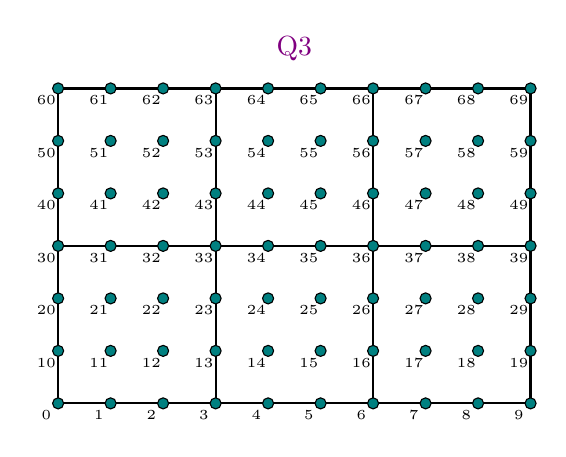
\begin{tikzpicture} 
\node[violet] at (3,4.5) {Q3}; 
\draw[thick] (0,0) -- (6,0) -- (6,4) -- (0,4) -- cycle; 
\draw[thick] (0,2) -- (6,2) ; 
\draw[thick] (2,0) -- (2,4) ; 
\draw[thick] (4,0) -- (4,4) ; 
\draw[black,fill=teal] ( 0.000000 , 0.000000)     circle (2pt); 
\node[] at ( -0.150000, -0.150000 ) {\tiny 0 }; 
\draw[black,fill=teal] ( 0.666667 , 0.000000)     circle (2pt); 
\node[] at ( 0.516667, -0.150000 ) {\tiny 1 }; 
\draw[black,fill=teal] ( 1.333333 , 0.000000)     circle (2pt); 
\node[] at ( 1.183333, -0.150000 ) {\tiny 2 }; 
\draw[black,fill=teal] ( 2.000000 , 0.000000)     circle (2pt); 
\node[] at ( 1.850000, -0.150000 ) {\tiny 3 }; 
\draw[black,fill=teal] ( 2.666667 , 0.000000)     circle (2pt); 
\node[] at ( 2.516667, -0.150000 ) {\tiny 4 }; 
\draw[black,fill=teal] ( 3.333333 , 0.000000)     circle (2pt); 
\node[] at ( 3.183333, -0.150000 ) {\tiny 5 }; 
\draw[black,fill=teal] ( 4.000000 , 0.000000)     circle (2pt); 
\node[] at ( 3.850000, -0.150000 ) {\tiny 6 }; 
\draw[black,fill=teal] ( 4.666667 , 0.000000)     circle (2pt); 
\node[] at ( 4.516667, -0.150000 ) {\tiny 7 }; 
\draw[black,fill=teal] ( 5.333333 , 0.000000)     circle (2pt); 
\node[] at ( 5.183333, -0.150000 ) {\tiny 8 }; 
\draw[black,fill=teal] ( 6.000000 , 0.000000)     circle (2pt); 
\node[] at ( 5.850000, -0.150000 ) {\tiny 9 }; 
\draw[black,fill=teal] ( 0.000000 , 0.666667)     circle (2pt); 
\node[] at ( -0.150000, 0.516667 ) {\tiny 10 }; 
\draw[black,fill=teal] ( 0.666667 , 0.666667)     circle (2pt); 
\node[] at ( 0.516667, 0.516667 ) {\tiny 11 }; 
\draw[black,fill=teal] ( 1.333333 , 0.666667)     circle (2pt); 
\node[] at ( 1.183333, 0.516667 ) {\tiny 12 }; 
\draw[black,fill=teal] ( 2.000000 , 0.666667)     circle (2pt); 
\node[] at ( 1.850000, 0.516667 ) {\tiny 13 }; 
\draw[black,fill=teal] ( 2.666667 , 0.666667)     circle (2pt); 
\node[] at ( 2.516667, 0.516667 ) {\tiny 14 }; 
\draw[black,fill=teal] ( 3.333333 , 0.666667)     circle (2pt); 
\node[] at ( 3.183333, 0.516667 ) {\tiny 15 }; 
\draw[black,fill=teal] ( 4.000000 , 0.666667)     circle (2pt); 
\node[] at ( 3.850000, 0.516667 ) {\tiny 16 }; 
\draw[black,fill=teal] ( 4.666667 , 0.666667)     circle (2pt); 
\node[] at ( 4.516667, 0.516667 ) {\tiny 17 }; 
\draw[black,fill=teal] ( 5.333333 , 0.666667)     circle (2pt); 
\node[] at ( 5.183333, 0.516667 ) {\tiny 18 }; 
\draw[black,fill=teal] ( 6.000000 , 0.666667)     circle (2pt); 
\node[] at ( 5.850000, 0.516667 ) {\tiny 19 }; 
\draw[black,fill=teal] ( 0.000000 , 1.333333)     circle (2pt); 
\node[] at ( -0.150000, 1.183333 ) {\tiny 20 }; 
\draw[black,fill=teal] ( 0.666667 , 1.333333)     circle (2pt); 
\node[] at ( 0.516667, 1.183333 ) {\tiny 21 }; 
\draw[black,fill=teal] ( 1.333333 , 1.333333)     circle (2pt); 
\node[] at ( 1.183333, 1.183333 ) {\tiny 22 }; 
\draw[black,fill=teal] ( 2.000000 , 1.333333)     circle (2pt); 
\node[] at ( 1.850000, 1.183333 ) {\tiny 23 }; 
\draw[black,fill=teal] ( 2.666667 , 1.333333)     circle (2pt); 
\node[] at ( 2.516667, 1.183333 ) {\tiny 24 }; 
\draw[black,fill=teal] ( 3.333333 , 1.333333)     circle (2pt); 
\node[] at ( 3.183333, 1.183333 ) {\tiny 25 }; 
\draw[black,fill=teal] ( 4.000000 , 1.333333)     circle (2pt); 
\node[] at ( 3.850000, 1.183333 ) {\tiny 26 }; 
\draw[black,fill=teal] ( 4.666667 , 1.333333)     circle (2pt); 
\node[] at ( 4.516667, 1.183333 ) {\tiny 27 }; 
\draw[black,fill=teal] ( 5.333333 , 1.333333)     circle (2pt); 
\node[] at ( 5.183333, 1.183333 ) {\tiny 28 }; 
\draw[black,fill=teal] ( 6.000000 , 1.333333)     circle (2pt); 
\node[] at ( 5.850000, 1.183333 ) {\tiny 29 }; 
\draw[black,fill=teal] ( 0.000000 , 2.000000)     circle (2pt); 
\node[] at ( -0.150000, 1.850000 ) {\tiny 30 }; 
\draw[black,fill=teal] ( 0.666667 , 2.000000)     circle (2pt); 
\node[] at ( 0.516667, 1.850000 ) {\tiny 31 }; 
\draw[black,fill=teal] ( 1.333333 , 2.000000)     circle (2pt); 
\node[] at ( 1.183333, 1.850000 ) {\tiny 32 }; 
\draw[black,fill=teal] ( 2.000000 , 2.000000)     circle (2pt); 
\node[] at ( 1.850000, 1.850000 ) {\tiny 33 }; 
\draw[black,fill=teal] ( 2.666667 , 2.000000)     circle (2pt); 
\node[] at ( 2.516667, 1.850000 ) {\tiny 34 }; 
\draw[black,fill=teal] ( 3.333333 , 2.000000)     circle (2pt); 
\node[] at ( 3.183333, 1.850000 ) {\tiny 35 }; 
\draw[black,fill=teal] ( 4.000000 , 2.000000)     circle (2pt); 
\node[] at ( 3.850000, 1.850000 ) {\tiny 36 }; 
\draw[black,fill=teal] ( 4.666667 , 2.000000)     circle (2pt); 
\node[] at ( 4.516667, 1.850000 ) {\tiny 37 }; 
\draw[black,fill=teal] ( 5.333333 , 2.000000)     circle (2pt); 
\node[] at ( 5.183333, 1.850000 ) {\tiny 38 }; 
\draw[black,fill=teal] ( 6.000000 , 2.000000)     circle (2pt); 
\node[] at ( 5.850000, 1.850000 ) {\tiny 39 }; 
\draw[black,fill=teal] ( 0.000000 , 2.666667)     circle (2pt); 
\node[] at ( -0.150000, 2.516667 ) {\tiny 40 }; 
\draw[black,fill=teal] ( 0.666667 , 2.666667)     circle (2pt); 
\node[] at ( 0.516667, 2.516667 ) {\tiny 41 }; 
\draw[black,fill=teal] ( 1.333333 , 2.666667)     circle (2pt); 
\node[] at ( 1.183333, 2.516667 ) {\tiny 42 }; 
\draw[black,fill=teal] ( 2.000000 , 2.666667)     circle (2pt); 
\node[] at ( 1.850000, 2.516667 ) {\tiny 43 }; 
\draw[black,fill=teal] ( 2.666667 , 2.666667)     circle (2pt); 
\node[] at ( 2.516667, 2.516667 ) {\tiny 44 }; 
\draw[black,fill=teal] ( 3.333333 , 2.666667)     circle (2pt); 
\node[] at ( 3.183333, 2.516667 ) {\tiny 45 }; 
\draw[black,fill=teal] ( 4.000000 , 2.666667)     circle (2pt); 
\node[] at ( 3.850000, 2.516667 ) {\tiny 46 }; 
\draw[black,fill=teal] ( 4.666667 , 2.666667)     circle (2pt); 
\node[] at ( 4.516667, 2.516667 ) {\tiny 47 }; 
\draw[black,fill=teal] ( 5.333333 , 2.666667)     circle (2pt); 
\node[] at ( 5.183333, 2.516667 ) {\tiny 48 }; 
\draw[black,fill=teal] ( 6.000000 , 2.666667)     circle (2pt); 
\node[] at ( 5.850000, 2.516667 ) {\tiny 49 }; 
\draw[black,fill=teal] ( 0.000000 , 3.333333)     circle (2pt); 
\node[] at ( -0.150000, 3.183333 ) {\tiny 50 }; 
\draw[black,fill=teal] ( 0.666667 , 3.333333)     circle (2pt); 
\node[] at ( 0.516667, 3.183333 ) {\tiny 51 }; 
\draw[black,fill=teal] ( 1.333333 , 3.333333)     circle (2pt); 
\node[] at ( 1.183333, 3.183333 ) {\tiny 52 }; 
\draw[black,fill=teal] ( 2.000000 , 3.333333)     circle (2pt); 
\node[] at ( 1.850000, 3.183333 ) {\tiny 53 }; 
\draw[black,fill=teal] ( 2.666667 , 3.333333)     circle (2pt); 
\node[] at ( 2.516667, 3.183333 ) {\tiny 54 }; 
\draw[black,fill=teal] ( 3.333333 , 3.333333)     circle (2pt); 
\node[] at ( 3.183333, 3.183333 ) {\tiny 55 }; 
\draw[black,fill=teal] ( 4.000000 , 3.333333)     circle (2pt); 
\node[] at ( 3.850000, 3.183333 ) {\tiny 56 }; 
\draw[black,fill=teal] ( 4.666667 , 3.333333)     circle (2pt); 
\node[] at ( 4.516667, 3.183333 ) {\tiny 57 }; 
\draw[black,fill=teal] ( 5.333333 , 3.333333)     circle (2pt); 
\node[] at ( 5.183333, 3.183333 ) {\tiny 58 }; 
\draw[black,fill=teal] ( 6.000000 , 3.333333)     circle (2pt); 
\node[] at ( 5.850000, 3.183333 ) {\tiny 59 }; 
\draw[black,fill=teal] ( 0.000000 , 4.000000)     circle (2pt); 
\node[] at ( -0.150000, 3.850000 ) {\tiny 60 }; 
\draw[black,fill=teal] ( 0.666667 , 4.000000)     circle (2pt); 
\node[] at ( 0.516667, 3.850000 ) {\tiny 61 }; 
\draw[black,fill=teal] ( 1.333333 , 4.000000)     circle (2pt); 
\node[] at ( 1.183333, 3.850000 ) {\tiny 62 }; 
\draw[black,fill=teal] ( 2.000000 , 4.000000)     circle (2pt); 
\node[] at ( 1.850000, 3.850000 ) {\tiny 63 }; 
\draw[black,fill=teal] ( 2.666667 , 4.000000)     circle (2pt); 
\node[] at ( 2.516667, 3.850000 ) {\tiny 64 }; 
\draw[black,fill=teal] ( 3.333333 , 4.000000)     circle (2pt); 
\node[] at ( 3.183333, 3.850000 ) {\tiny 65 }; 
\draw[black,fill=teal] ( 4.000000 , 4.000000)     circle (2pt); 
\node[] at ( 3.850000, 3.850000 ) {\tiny 66 }; 
\draw[black,fill=teal] ( 4.666667 , 4.000000)     circle (2pt); 
\node[] at ( 4.516667, 3.850000 ) {\tiny 67 }; 
\draw[black,fill=teal] ( 5.333333 , 4.000000)     circle (2pt); 
\node[] at ( 5.183333, 3.850000 ) {\tiny 68 }; 
\draw[black,fill=teal] ( 6.000000 , 4.000000)     circle (2pt); 
\node[] at ( 5.850000, 3.850000 ) {\tiny 69 }; 
\end{tikzpicture} 
\end{center} 


%--------------------------------
\begin{center} 
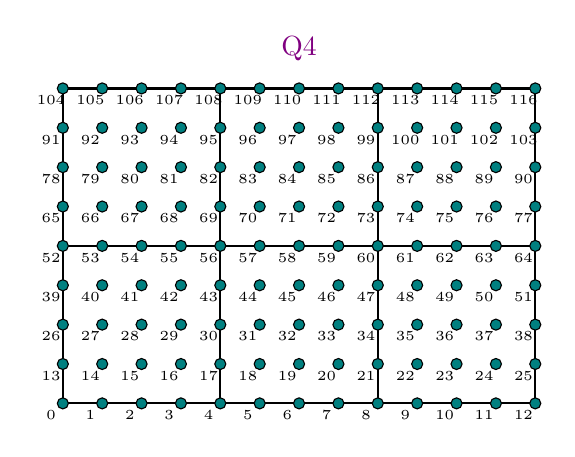
\begin{tikzpicture} 
\node[violet] at (3,4.5) {Q4}; 
\draw[thick] (0,0) -- (6,0) -- (6,4) -- (0,4) -- cycle; 
\draw[thick] (0,2) -- (6,2) ; 
\draw[thick] (2,0) -- (2,4) ; 
\draw[thick] (4,0) -- (4,4) ; 
\draw[black,fill=teal] ( 0.000000 , 0.000000)     circle (2pt); 
\node[] at ( -0.150000, -0.150000 ) {\tiny 0 }; 
\draw[black,fill=teal] ( 0.500000 , 0.000000)     circle (2pt); 
\node[] at ( 0.350000, -0.150000 ) {\tiny 1 }; 
\draw[black,fill=teal] ( 1.000000 , 0.000000)     circle (2pt); 
\node[] at ( 0.850000, -0.150000 ) {\tiny 2 }; 
\draw[black,fill=teal] ( 1.500000 , 0.000000)     circle (2pt); 
\node[] at ( 1.350000, -0.150000 ) {\tiny 3 }; 
\draw[black,fill=teal] ( 2.000000 , 0.000000)     circle (2pt); 
\node[] at ( 1.850000, -0.150000 ) {\tiny 4 }; 
\draw[black,fill=teal] ( 2.500000 , 0.000000)     circle (2pt); 
\node[] at ( 2.350000, -0.150000 ) {\tiny 5 }; 
\draw[black,fill=teal] ( 3.000000 , 0.000000)     circle (2pt); 
\node[] at ( 2.850000, -0.150000 ) {\tiny 6 }; 
\draw[black,fill=teal] ( 3.500000 , 0.000000)     circle (2pt); 
\node[] at ( 3.350000, -0.150000 ) {\tiny 7 }; 
\draw[black,fill=teal] ( 4.000000 , 0.000000)     circle (2pt); 
\node[] at ( 3.850000, -0.150000 ) {\tiny 8 }; 
\draw[black,fill=teal] ( 4.500000 , 0.000000)     circle (2pt); 
\node[] at ( 4.350000, -0.150000 ) {\tiny 9 }; 
\draw[black,fill=teal] ( 5.000000 , 0.000000)     circle (2pt); 
\node[] at ( 4.850000, -0.150000 ) {\tiny 10 }; 
\draw[black,fill=teal] ( 5.500000 , 0.000000)     circle (2pt); 
\node[] at ( 5.350000, -0.150000 ) {\tiny 11 }; 
\draw[black,fill=teal] ( 6.000000 , 0.000000)     circle (2pt); 
\node[] at ( 5.850000, -0.150000 ) {\tiny 12 }; 
\draw[black,fill=teal] ( 0.000000 , 0.500000)     circle (2pt); 
\node[] at ( -0.150000, 0.350000 ) {\tiny 13 }; 
\draw[black,fill=teal] ( 0.500000 , 0.500000)     circle (2pt); 
\node[] at ( 0.350000, 0.350000 ) {\tiny 14 }; 
\draw[black,fill=teal] ( 1.000000 , 0.500000)     circle (2pt); 
\node[] at ( 0.850000, 0.350000 ) {\tiny 15 }; 
\draw[black,fill=teal] ( 1.500000 , 0.500000)     circle (2pt); 
\node[] at ( 1.350000, 0.350000 ) {\tiny 16 }; 
\draw[black,fill=teal] ( 2.000000 , 0.500000)     circle (2pt); 
\node[] at ( 1.850000, 0.350000 ) {\tiny 17 }; 
\draw[black,fill=teal] ( 2.500000 , 0.500000)     circle (2pt); 
\node[] at ( 2.350000, 0.350000 ) {\tiny 18 }; 
\draw[black,fill=teal] ( 3.000000 , 0.500000)     circle (2pt); 
\node[] at ( 2.850000, 0.350000 ) {\tiny 19 }; 
\draw[black,fill=teal] ( 3.500000 , 0.500000)     circle (2pt); 
\node[] at ( 3.350000, 0.350000 ) {\tiny 20 }; 
\draw[black,fill=teal] ( 4.000000 , 0.500000)     circle (2pt); 
\node[] at ( 3.850000, 0.350000 ) {\tiny 21 }; 
\draw[black,fill=teal] ( 4.500000 , 0.500000)     circle (2pt); 
\node[] at ( 4.350000, 0.350000 ) {\tiny 22 }; 
\draw[black,fill=teal] ( 5.000000 , 0.500000)     circle (2pt); 
\node[] at ( 4.850000, 0.350000 ) {\tiny 23 }; 
\draw[black,fill=teal] ( 5.500000 , 0.500000)     circle (2pt); 
\node[] at ( 5.350000, 0.350000 ) {\tiny 24 }; 
\draw[black,fill=teal] ( 6.000000 , 0.500000)     circle (2pt); 
\node[] at ( 5.850000, 0.350000 ) {\tiny 25 }; 
\draw[black,fill=teal] ( 0.000000 , 1.000000)     circle (2pt); 
\node[] at ( -0.150000, 0.850000 ) {\tiny 26 }; 
\draw[black,fill=teal] ( 0.500000 , 1.000000)     circle (2pt); 
\node[] at ( 0.350000, 0.850000 ) {\tiny 27 }; 
\draw[black,fill=teal] ( 1.000000 , 1.000000)     circle (2pt); 
\node[] at ( 0.850000, 0.850000 ) {\tiny 28 }; 
\draw[black,fill=teal] ( 1.500000 , 1.000000)     circle (2pt); 
\node[] at ( 1.350000, 0.850000 ) {\tiny 29 }; 
\draw[black,fill=teal] ( 2.000000 , 1.000000)     circle (2pt); 
\node[] at ( 1.850000, 0.850000 ) {\tiny 30 }; 
\draw[black,fill=teal] ( 2.500000 , 1.000000)     circle (2pt); 
\node[] at ( 2.350000, 0.850000 ) {\tiny 31 }; 
\draw[black,fill=teal] ( 3.000000 , 1.000000)     circle (2pt); 
\node[] at ( 2.850000, 0.850000 ) {\tiny 32 }; 
\draw[black,fill=teal] ( 3.500000 , 1.000000)     circle (2pt); 
\node[] at ( 3.350000, 0.850000 ) {\tiny 33 }; 
\draw[black,fill=teal] ( 4.000000 , 1.000000)     circle (2pt); 
\node[] at ( 3.850000, 0.850000 ) {\tiny 34 }; 
\draw[black,fill=teal] ( 4.500000 , 1.000000)     circle (2pt); 
\node[] at ( 4.350000, 0.850000 ) {\tiny 35 }; 
\draw[black,fill=teal] ( 5.000000 , 1.000000)     circle (2pt); 
\node[] at ( 4.850000, 0.850000 ) {\tiny 36 }; 
\draw[black,fill=teal] ( 5.500000 , 1.000000)     circle (2pt); 
\node[] at ( 5.350000, 0.850000 ) {\tiny 37 }; 
\draw[black,fill=teal] ( 6.000000 , 1.000000)     circle (2pt); 
\node[] at ( 5.850000, 0.850000 ) {\tiny 38 }; 
\draw[black,fill=teal] ( 0.000000 , 1.500000)     circle (2pt); 
\node[] at ( -0.150000, 1.350000 ) {\tiny 39 }; 
\draw[black,fill=teal] ( 0.500000 , 1.500000)     circle (2pt); 
\node[] at ( 0.350000, 1.350000 ) {\tiny 40 }; 
\draw[black,fill=teal] ( 1.000000 , 1.500000)     circle (2pt); 
\node[] at ( 0.850000, 1.350000 ) {\tiny 41 }; 
\draw[black,fill=teal] ( 1.500000 , 1.500000)     circle (2pt); 
\node[] at ( 1.350000, 1.350000 ) {\tiny 42 }; 
\draw[black,fill=teal] ( 2.000000 , 1.500000)     circle (2pt); 
\node[] at ( 1.850000, 1.350000 ) {\tiny 43 }; 
\draw[black,fill=teal] ( 2.500000 , 1.500000)     circle (2pt); 
\node[] at ( 2.350000, 1.350000 ) {\tiny 44 }; 
\draw[black,fill=teal] ( 3.000000 , 1.500000)     circle (2pt); 
\node[] at ( 2.850000, 1.350000 ) {\tiny 45 }; 
\draw[black,fill=teal] ( 3.500000 , 1.500000)     circle (2pt); 
\node[] at ( 3.350000, 1.350000 ) {\tiny 46 }; 
\draw[black,fill=teal] ( 4.000000 , 1.500000)     circle (2pt); 
\node[] at ( 3.850000, 1.350000 ) {\tiny 47 }; 
\draw[black,fill=teal] ( 4.500000 , 1.500000)     circle (2pt); 
\node[] at ( 4.350000, 1.350000 ) {\tiny 48 }; 
\draw[black,fill=teal] ( 5.000000 , 1.500000)     circle (2pt); 
\node[] at ( 4.850000, 1.350000 ) {\tiny 49 }; 
\draw[black,fill=teal] ( 5.500000 , 1.500000)     circle (2pt); 
\node[] at ( 5.350000, 1.350000 ) {\tiny 50 }; 
\draw[black,fill=teal] ( 6.000000 , 1.500000)     circle (2pt); 
\node[] at ( 5.850000, 1.350000 ) {\tiny 51 }; 
\draw[black,fill=teal] ( 0.000000 , 2.000000)     circle (2pt); 
\node[] at ( -0.150000, 1.850000 ) {\tiny 52 }; 
\draw[black,fill=teal] ( 0.500000 , 2.000000)     circle (2pt); 
\node[] at ( 0.350000, 1.850000 ) {\tiny 53 }; 
\draw[black,fill=teal] ( 1.000000 , 2.000000)     circle (2pt); 
\node[] at ( 0.850000, 1.850000 ) {\tiny 54 }; 
\draw[black,fill=teal] ( 1.500000 , 2.000000)     circle (2pt); 
\node[] at ( 1.350000, 1.850000 ) {\tiny 55 }; 
\draw[black,fill=teal] ( 2.000000 , 2.000000)     circle (2pt); 
\node[] at ( 1.850000, 1.850000 ) {\tiny 56 }; 
\draw[black,fill=teal] ( 2.500000 , 2.000000)     circle (2pt); 
\node[] at ( 2.350000, 1.850000 ) {\tiny 57 }; 
\draw[black,fill=teal] ( 3.000000 , 2.000000)     circle (2pt); 
\node[] at ( 2.850000, 1.850000 ) {\tiny 58 }; 
\draw[black,fill=teal] ( 3.500000 , 2.000000)     circle (2pt); 
\node[] at ( 3.350000, 1.850000 ) {\tiny 59 }; 
\draw[black,fill=teal] ( 4.000000 , 2.000000)     circle (2pt); 
\node[] at ( 3.850000, 1.850000 ) {\tiny 60 }; 
\draw[black,fill=teal] ( 4.500000 , 2.000000)     circle (2pt); 
\node[] at ( 4.350000, 1.850000 ) {\tiny 61 }; 
\draw[black,fill=teal] ( 5.000000 , 2.000000)     circle (2pt); 
\node[] at ( 4.850000, 1.850000 ) {\tiny 62 }; 
\draw[black,fill=teal] ( 5.500000 , 2.000000)     circle (2pt); 
\node[] at ( 5.350000, 1.850000 ) {\tiny 63 }; 
\draw[black,fill=teal] ( 6.000000 , 2.000000)     circle (2pt); 
\node[] at ( 5.850000, 1.850000 ) {\tiny 64 }; 
\draw[black,fill=teal] ( 0.000000 , 2.500000)     circle (2pt); 
\node[] at ( -0.150000, 2.350000 ) {\tiny 65 }; 
\draw[black,fill=teal] ( 0.500000 , 2.500000)     circle (2pt); 
\node[] at ( 0.350000, 2.350000 ) {\tiny 66 }; 
\draw[black,fill=teal] ( 1.000000 , 2.500000)     circle (2pt); 
\node[] at ( 0.850000, 2.350000 ) {\tiny 67 }; 
\draw[black,fill=teal] ( 1.500000 , 2.500000)     circle (2pt); 
\node[] at ( 1.350000, 2.350000 ) {\tiny 68 }; 
\draw[black,fill=teal] ( 2.000000 , 2.500000)     circle (2pt); 
\node[] at ( 1.850000, 2.350000 ) {\tiny 69 }; 
\draw[black,fill=teal] ( 2.500000 , 2.500000)     circle (2pt); 
\node[] at ( 2.350000, 2.350000 ) {\tiny 70 }; 
\draw[black,fill=teal] ( 3.000000 , 2.500000)     circle (2pt); 
\node[] at ( 2.850000, 2.350000 ) {\tiny 71 }; 
\draw[black,fill=teal] ( 3.500000 , 2.500000)     circle (2pt); 
\node[] at ( 3.350000, 2.350000 ) {\tiny 72 }; 
\draw[black,fill=teal] ( 4.000000 , 2.500000)     circle (2pt); 
\node[] at ( 3.850000, 2.350000 ) {\tiny 73 }; 
\draw[black,fill=teal] ( 4.500000 , 2.500000)     circle (2pt); 
\node[] at ( 4.350000, 2.350000 ) {\tiny 74 }; 
\draw[black,fill=teal] ( 5.000000 , 2.500000)     circle (2pt); 
\node[] at ( 4.850000, 2.350000 ) {\tiny 75 }; 
\draw[black,fill=teal] ( 5.500000 , 2.500000)     circle (2pt); 
\node[] at ( 5.350000, 2.350000 ) {\tiny 76 }; 
\draw[black,fill=teal] ( 6.000000 , 2.500000)     circle (2pt); 
\node[] at ( 5.850000, 2.350000 ) {\tiny 77 }; 
\draw[black,fill=teal] ( 0.000000 , 3.000000)     circle (2pt); 
\node[] at ( -0.150000, 2.850000 ) {\tiny 78 }; 
\draw[black,fill=teal] ( 0.500000 , 3.000000)     circle (2pt); 
\node[] at ( 0.350000, 2.850000 ) {\tiny 79 }; 
\draw[black,fill=teal] ( 1.000000 , 3.000000)     circle (2pt); 
\node[] at ( 0.850000, 2.850000 ) {\tiny 80 }; 
\draw[black,fill=teal] ( 1.500000 , 3.000000)     circle (2pt); 
\node[] at ( 1.350000, 2.850000 ) {\tiny 81 }; 
\draw[black,fill=teal] ( 2.000000 , 3.000000)     circle (2pt); 
\node[] at ( 1.850000, 2.850000 ) {\tiny 82 }; 
\draw[black,fill=teal] ( 2.500000 , 3.000000)     circle (2pt); 
\node[] at ( 2.350000, 2.850000 ) {\tiny 83 }; 
\draw[black,fill=teal] ( 3.000000 , 3.000000)     circle (2pt); 
\node[] at ( 2.850000, 2.850000 ) {\tiny 84 }; 
\draw[black,fill=teal] ( 3.500000 , 3.000000)     circle (2pt); 
\node[] at ( 3.350000, 2.850000 ) {\tiny 85 }; 
\draw[black,fill=teal] ( 4.000000 , 3.000000)     circle (2pt); 
\node[] at ( 3.850000, 2.850000 ) {\tiny 86 }; 
\draw[black,fill=teal] ( 4.500000 , 3.000000)     circle (2pt); 
\node[] at ( 4.350000, 2.850000 ) {\tiny 87 }; 
\draw[black,fill=teal] ( 5.000000 , 3.000000)     circle (2pt); 
\node[] at ( 4.850000, 2.850000 ) {\tiny 88 }; 
\draw[black,fill=teal] ( 5.500000 , 3.000000)     circle (2pt); 
\node[] at ( 5.350000, 2.850000 ) {\tiny 89 }; 
\draw[black,fill=teal] ( 6.000000 , 3.000000)     circle (2pt); 
\node[] at ( 5.850000, 2.850000 ) {\tiny 90 }; 
\draw[black,fill=teal] ( 0.000000 , 3.500000)     circle (2pt); 
\node[] at ( -0.150000, 3.350000 ) {\tiny 91 }; 
\draw[black,fill=teal] ( 0.500000 , 3.500000)     circle (2pt); 
\node[] at ( 0.350000, 3.350000 ) {\tiny 92 }; 
\draw[black,fill=teal] ( 1.000000 , 3.500000)     circle (2pt); 
\node[] at ( 0.850000, 3.350000 ) {\tiny 93 }; 
\draw[black,fill=teal] ( 1.500000 , 3.500000)     circle (2pt); 
\node[] at ( 1.350000, 3.350000 ) {\tiny 94 }; 
\draw[black,fill=teal] ( 2.000000 , 3.500000)     circle (2pt); 
\node[] at ( 1.850000, 3.350000 ) {\tiny 95 }; 
\draw[black,fill=teal] ( 2.500000 , 3.500000)     circle (2pt); 
\node[] at ( 2.350000, 3.350000 ) {\tiny 96 }; 
\draw[black,fill=teal] ( 3.000000 , 3.500000)     circle (2pt); 
\node[] at ( 2.850000, 3.350000 ) {\tiny 97 }; 
\draw[black,fill=teal] ( 3.500000 , 3.500000)     circle (2pt); 
\node[] at ( 3.350000, 3.350000 ) {\tiny 98 }; 
\draw[black,fill=teal] ( 4.000000 , 3.500000)     circle (2pt); 
\node[] at ( 3.850000, 3.350000 ) {\tiny 99 }; 
\draw[black,fill=teal] ( 4.500000 , 3.500000)     circle (2pt); 
\node[] at ( 4.350000, 3.350000 ) {\tiny 100 }; 
\draw[black,fill=teal] ( 5.000000 , 3.500000)     circle (2pt); 
\node[] at ( 4.850000, 3.350000 ) {\tiny 101 }; 
\draw[black,fill=teal] ( 5.500000 , 3.500000)     circle (2pt); 
\node[] at ( 5.350000, 3.350000 ) {\tiny 102 }; 
\draw[black,fill=teal] ( 6.000000 , 3.500000)     circle (2pt); 
\node[] at ( 5.850000, 3.350000 ) {\tiny 103 }; 
\draw[black,fill=teal] ( 0.000000 , 4.000000)     circle (2pt); 
\node[] at ( -0.150000, 3.850000 ) {\tiny 104 }; 
\draw[black,fill=teal] ( 0.500000 , 4.000000)     circle (2pt); 
\node[] at ( 0.350000, 3.850000 ) {\tiny 105 }; 
\draw[black,fill=teal] ( 1.000000 , 4.000000)     circle (2pt); 
\node[] at ( 0.850000, 3.850000 ) {\tiny 106 }; 
\draw[black,fill=teal] ( 1.500000 , 4.000000)     circle (2pt); 
\node[] at ( 1.350000, 3.850000 ) {\tiny 107 }; 
\draw[black,fill=teal] ( 2.000000 , 4.000000)     circle (2pt); 
\node[] at ( 1.850000, 3.850000 ) {\tiny 108 }; 
\draw[black,fill=teal] ( 2.500000 , 4.000000)     circle (2pt); 
\node[] at ( 2.350000, 3.850000 ) {\tiny 109 }; 
\draw[black,fill=teal] ( 3.000000 , 4.000000)     circle (2pt); 
\node[] at ( 2.850000, 3.850000 ) {\tiny 110 }; 
\draw[black,fill=teal] ( 3.500000 , 4.000000)     circle (2pt); 
\node[] at ( 3.350000, 3.850000 ) {\tiny 111 }; 
\draw[black,fill=teal] ( 4.000000 , 4.000000)     circle (2pt); 
\node[] at ( 3.850000, 3.850000 ) {\tiny 112 }; 
\draw[black,fill=teal] ( 4.500000 , 4.000000)     circle (2pt); 
\node[] at ( 4.350000, 3.850000 ) {\tiny 113 }; 
\draw[black,fill=teal] ( 5.000000 , 4.000000)     circle (2pt); 
\node[] at ( 4.850000, 3.850000 ) {\tiny 114 }; 
\draw[black,fill=teal] ( 5.500000 , 4.000000)     circle (2pt); 
\node[] at ( 5.350000, 3.850000 ) {\tiny 115 }; 
\draw[black,fill=teal] ( 6.000000 , 4.000000)     circle (2pt); 
\node[] at ( 5.850000, 3.850000 ) {\tiny 116 }; 
\end{tikzpicture} 
\end{center} 


%--------------------------------
\begin{center} 
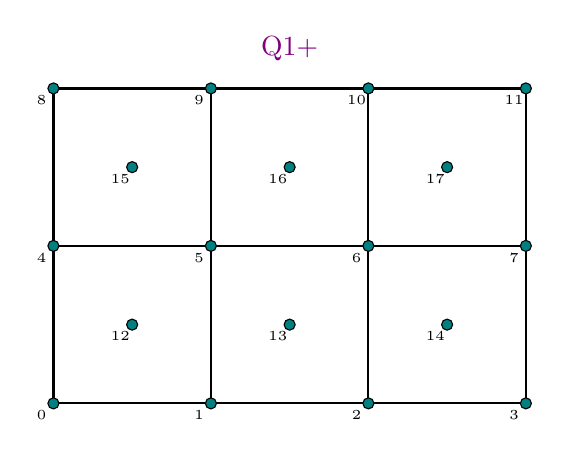
\begin{tikzpicture} 
\node[violet] at (3,4.5) {Q1+}; 
\draw[thick] (0,0) -- (6,0) -- (6,4) -- (0,4) -- cycle; 
\draw[thick] (0,2) -- (6,2) ; 
\draw[thick] (2,0) -- (2,4) ; 
\draw[thick] (4,0) -- (4,4) ; 
\draw[black,fill=teal] ( 0.000000 , 0.000000)     circle (2pt); 
\node[] at ( -0.150000, -0.150000 ) {\tiny 0 }; 
\draw[black,fill=teal] ( 2.000000 , 0.000000)     circle (2pt); 
\node[] at ( 1.850000, -0.150000 ) {\tiny 1 }; 
\draw[black,fill=teal] ( 4.000000 , 0.000000)     circle (2pt); 
\node[] at ( 3.850000, -0.150000 ) {\tiny 2 }; 
\draw[black,fill=teal] ( 6.000000 , 0.000000)     circle (2pt); 
\node[] at ( 5.850000, -0.150000 ) {\tiny 3 }; 
\draw[black,fill=teal] ( 0.000000 , 2.000000)     circle (2pt); 
\node[] at ( -0.150000, 1.850000 ) {\tiny 4 }; 
\draw[black,fill=teal] ( 2.000000 , 2.000000)     circle (2pt); 
\node[] at ( 1.850000, 1.850000 ) {\tiny 5 }; 
\draw[black,fill=teal] ( 4.000000 , 2.000000)     circle (2pt); 
\node[] at ( 3.850000, 1.850000 ) {\tiny 6 }; 
\draw[black,fill=teal] ( 6.000000 , 2.000000)     circle (2pt); 
\node[] at ( 5.850000, 1.850000 ) {\tiny 7 }; 
\draw[black,fill=teal] ( 0.000000 , 4.000000)     circle (2pt); 
\node[] at ( -0.150000, 3.850000 ) {\tiny 8 }; 
\draw[black,fill=teal] ( 2.000000 , 4.000000)     circle (2pt); 
\node[] at ( 1.850000, 3.850000 ) {\tiny 9 }; 
\draw[black,fill=teal] ( 4.000000 , 4.000000)     circle (2pt); 
\node[] at ( 3.850000, 3.850000 ) {\tiny 10 }; 
\draw[black,fill=teal] ( 6.000000 , 4.000000)     circle (2pt); 
\node[] at ( 5.850000, 3.850000 ) {\tiny 11 }; 
\draw[black,fill=teal] ( 1.000000 , 1.000000)     circle (2pt); 
\node[] at ( 0.850000, 0.850000 ) {\tiny 12 }; 
\draw[black,fill=teal] ( 3.000000 , 1.000000)     circle (2pt); 
\node[] at ( 2.850000, 0.850000 ) {\tiny 13 }; 
\draw[black,fill=teal] ( 5.000000 , 1.000000)     circle (2pt); 
\node[] at ( 4.850000, 0.850000 ) {\tiny 14 }; 
\draw[black,fill=teal] ( 1.000000 , 3.000000)     circle (2pt); 
\node[] at ( 0.850000, 2.850000 ) {\tiny 15 }; 
\draw[black,fill=teal] ( 3.000000 , 3.000000)     circle (2pt); 
\node[] at ( 2.850000, 2.850000 ) {\tiny 16 }; 
\draw[black,fill=teal] ( 5.000000 , 3.000000)     circle (2pt); 
\node[] at ( 4.850000, 2.850000 ) {\tiny 17 }; 
\end{tikzpicture} 
\end{center} 


%--------------------------------
\begin{center} 
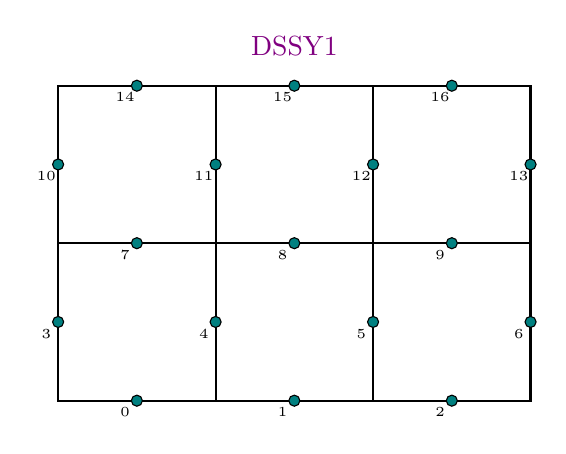
\begin{tikzpicture} 
\node[violet] at (3,4.5) {DSSY1}; 
\draw[thick] (0,0) -- (6,0) -- (6,4) -- (0,4) -- cycle; 
\draw[thick] (0,2) -- (6,2) ; 
\draw[thick] (2,0) -- (2,4) ; 
\draw[thick] (4,0) -- (4,4) ; 
\draw[black,fill=teal] ( 1.000000 , 0.000000)     circle (2pt); 
\node[] at ( 0.850000, -0.150000 ) {\tiny 0 }; 
\draw[black,fill=teal] ( 3.000000 , 0.000000)     circle (2pt); 
\node[] at ( 2.850000, -0.150000 ) {\tiny 1 }; 
\draw[black,fill=teal] ( 5.000000 , 0.000000)     circle (2pt); 
\node[] at ( 4.850000, -0.150000 ) {\tiny 2 }; 
\draw[black,fill=teal] ( 0.000000 , 1.000000)     circle (2pt); 
\node[] at ( -0.150000, 0.850000 ) {\tiny 3 }; 
\draw[black,fill=teal] ( 2.000000 , 1.000000)     circle (2pt); 
\node[] at ( 1.850000, 0.850000 ) {\tiny 4 }; 
\draw[black,fill=teal] ( 4.000000 , 1.000000)     circle (2pt); 
\node[] at ( 3.850000, 0.850000 ) {\tiny 5 }; 
\draw[black,fill=teal] ( 6.000000 , 1.000000)     circle (2pt); 
\node[] at ( 5.850000, 0.850000 ) {\tiny 6 }; 
\draw[black,fill=teal] ( 1.000000 , 2.000000)     circle (2pt); 
\node[] at ( 0.850000, 1.850000 ) {\tiny 7 }; 
\draw[black,fill=teal] ( 3.000000 , 2.000000)     circle (2pt); 
\node[] at ( 2.850000, 1.850000 ) {\tiny 8 }; 
\draw[black,fill=teal] ( 5.000000 , 2.000000)     circle (2pt); 
\node[] at ( 4.850000, 1.850000 ) {\tiny 9 }; 
\draw[black,fill=teal] ( 0.000000 , 3.000000)     circle (2pt); 
\node[] at ( -0.150000, 2.850000 ) {\tiny 10 }; 
\draw[black,fill=teal] ( 2.000000 , 3.000000)     circle (2pt); 
\node[] at ( 1.850000, 2.850000 ) {\tiny 11 }; 
\draw[black,fill=teal] ( 4.000000 , 3.000000)     circle (2pt); 
\node[] at ( 3.850000, 2.850000 ) {\tiny 12 }; 
\draw[black,fill=teal] ( 6.000000 , 3.000000)     circle (2pt); 
\node[] at ( 5.850000, 2.850000 ) {\tiny 13 }; 
\draw[black,fill=teal] ( 1.000000 , 4.000000)     circle (2pt); 
\node[] at ( 0.850000, 3.850000 ) {\tiny 14 }; 
\draw[black,fill=teal] ( 3.000000 , 4.000000)     circle (2pt); 
\node[] at ( 2.850000, 3.850000 ) {\tiny 15 }; 
\draw[black,fill=teal] ( 5.000000 , 4.000000)     circle (2pt); 
\node[] at ( 4.850000, 3.850000 ) {\tiny 16 }; 
\end{tikzpicture} 
\end{center} 


%--------------------------------
\begin{center} 
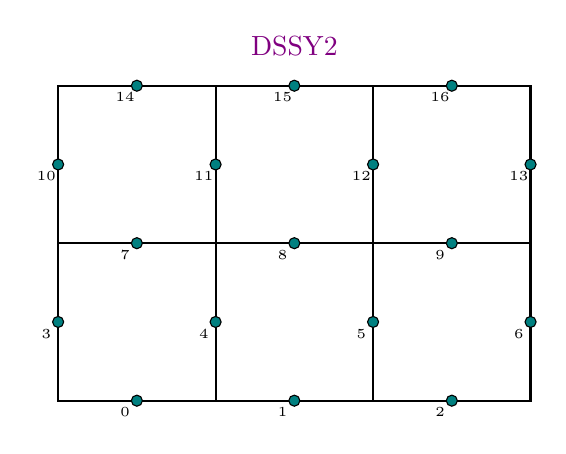
\begin{tikzpicture} 
\node[violet] at (3,4.5) {DSSY2}; 
\draw[thick] (0,0) -- (6,0) -- (6,4) -- (0,4) -- cycle; 
\draw[thick] (0,2) -- (6,2) ; 
\draw[thick] (2,0) -- (2,4) ; 
\draw[thick] (4,0) -- (4,4) ; 
\draw[black,fill=teal] ( 1.000000 , 0.000000)     circle (2pt); 
\node[] at ( 0.850000, -0.150000 ) {\tiny 0 }; 
\draw[black,fill=teal] ( 3.000000 , 0.000000)     circle (2pt); 
\node[] at ( 2.850000, -0.150000 ) {\tiny 1 }; 
\draw[black,fill=teal] ( 5.000000 , 0.000000)     circle (2pt); 
\node[] at ( 4.850000, -0.150000 ) {\tiny 2 }; 
\draw[black,fill=teal] ( 0.000000 , 1.000000)     circle (2pt); 
\node[] at ( -0.150000, 0.850000 ) {\tiny 3 }; 
\draw[black,fill=teal] ( 2.000000 , 1.000000)     circle (2pt); 
\node[] at ( 1.850000, 0.850000 ) {\tiny 4 }; 
\draw[black,fill=teal] ( 4.000000 , 1.000000)     circle (2pt); 
\node[] at ( 3.850000, 0.850000 ) {\tiny 5 }; 
\draw[black,fill=teal] ( 6.000000 , 1.000000)     circle (2pt); 
\node[] at ( 5.850000, 0.850000 ) {\tiny 6 }; 
\draw[black,fill=teal] ( 1.000000 , 2.000000)     circle (2pt); 
\node[] at ( 0.850000, 1.850000 ) {\tiny 7 }; 
\draw[black,fill=teal] ( 3.000000 , 2.000000)     circle (2pt); 
\node[] at ( 2.850000, 1.850000 ) {\tiny 8 }; 
\draw[black,fill=teal] ( 5.000000 , 2.000000)     circle (2pt); 
\node[] at ( 4.850000, 1.850000 ) {\tiny 9 }; 
\draw[black,fill=teal] ( 0.000000 , 3.000000)     circle (2pt); 
\node[] at ( -0.150000, 2.850000 ) {\tiny 10 }; 
\draw[black,fill=teal] ( 2.000000 , 3.000000)     circle (2pt); 
\node[] at ( 1.850000, 2.850000 ) {\tiny 11 }; 
\draw[black,fill=teal] ( 4.000000 , 3.000000)     circle (2pt); 
\node[] at ( 3.850000, 2.850000 ) {\tiny 12 }; 
\draw[black,fill=teal] ( 6.000000 , 3.000000)     circle (2pt); 
\node[] at ( 5.850000, 2.850000 ) {\tiny 13 }; 
\draw[black,fill=teal] ( 1.000000 , 4.000000)     circle (2pt); 
\node[] at ( 0.850000, 3.850000 ) {\tiny 14 }; 
\draw[black,fill=teal] ( 3.000000 , 4.000000)     circle (2pt); 
\node[] at ( 2.850000, 3.850000 ) {\tiny 15 }; 
\draw[black,fill=teal] ( 5.000000 , 4.000000)     circle (2pt); 
\node[] at ( 4.850000, 3.850000 ) {\tiny 16 }; 
\end{tikzpicture} 
\end{center} 


%--------------------------------
\begin{center} 
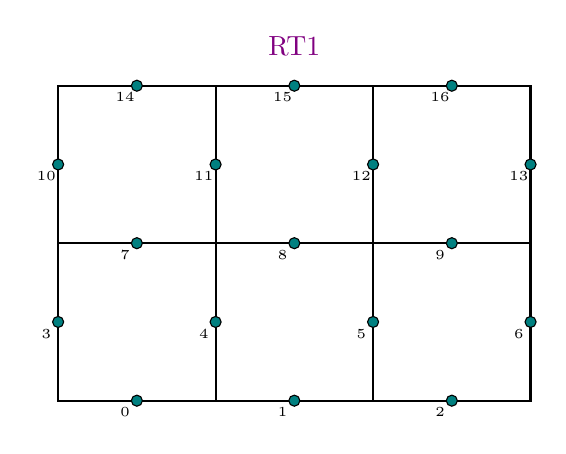
\begin{tikzpicture} 
\node[violet] at (3,4.5) {RT1}; 
\draw[thick] (0,0) -- (6,0) -- (6,4) -- (0,4) -- cycle; 
\draw[thick] (0,2) -- (6,2) ; 
\draw[thick] (2,0) -- (2,4) ; 
\draw[thick] (4,0) -- (4,4) ; 
\draw[black,fill=teal] ( 1.000000 , 0.000000)     circle (2pt); 
\node[] at ( 0.850000, -0.150000 ) {\tiny 0 }; 
\draw[black,fill=teal] ( 3.000000 , 0.000000)     circle (2pt); 
\node[] at ( 2.850000, -0.150000 ) {\tiny 1 }; 
\draw[black,fill=teal] ( 5.000000 , 0.000000)     circle (2pt); 
\node[] at ( 4.850000, -0.150000 ) {\tiny 2 }; 
\draw[black,fill=teal] ( 0.000000 , 1.000000)     circle (2pt); 
\node[] at ( -0.150000, 0.850000 ) {\tiny 3 }; 
\draw[black,fill=teal] ( 2.000000 , 1.000000)     circle (2pt); 
\node[] at ( 1.850000, 0.850000 ) {\tiny 4 }; 
\draw[black,fill=teal] ( 4.000000 , 1.000000)     circle (2pt); 
\node[] at ( 3.850000, 0.850000 ) {\tiny 5 }; 
\draw[black,fill=teal] ( 6.000000 , 1.000000)     circle (2pt); 
\node[] at ( 5.850000, 0.850000 ) {\tiny 6 }; 
\draw[black,fill=teal] ( 1.000000 , 2.000000)     circle (2pt); 
\node[] at ( 0.850000, 1.850000 ) {\tiny 7 }; 
\draw[black,fill=teal] ( 3.000000 , 2.000000)     circle (2pt); 
\node[] at ( 2.850000, 1.850000 ) {\tiny 8 }; 
\draw[black,fill=teal] ( 5.000000 , 2.000000)     circle (2pt); 
\node[] at ( 4.850000, 1.850000 ) {\tiny 9 }; 
\draw[black,fill=teal] ( 0.000000 , 3.000000)     circle (2pt); 
\node[] at ( -0.150000, 2.850000 ) {\tiny 10 }; 
\draw[black,fill=teal] ( 2.000000 , 3.000000)     circle (2pt); 
\node[] at ( 1.850000, 2.850000 ) {\tiny 11 }; 
\draw[black,fill=teal] ( 4.000000 , 3.000000)     circle (2pt); 
\node[] at ( 3.850000, 2.850000 ) {\tiny 12 }; 
\draw[black,fill=teal] ( 6.000000 , 3.000000)     circle (2pt); 
\node[] at ( 5.850000, 2.850000 ) {\tiny 13 }; 
\draw[black,fill=teal] ( 1.000000 , 4.000000)     circle (2pt); 
\node[] at ( 0.850000, 3.850000 ) {\tiny 14 }; 
\draw[black,fill=teal] ( 3.000000 , 4.000000)     circle (2pt); 
\node[] at ( 2.850000, 3.850000 ) {\tiny 15 }; 
\draw[black,fill=teal] ( 5.000000 , 4.000000)     circle (2pt); 
\node[] at ( 4.850000, 3.850000 ) {\tiny 16 }; 
\end{tikzpicture} 
\end{center} 


%--------------------------------
\begin{center} 
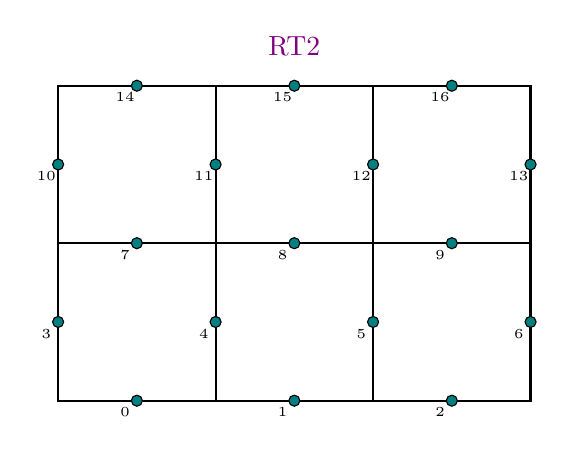
\begin{tikzpicture} 
\node[violet] at (3,4.5) {RT2}; 
\draw[thick] (0,0) -- (6,0) -- (6,4) -- (0,4) -- cycle; 
\draw[thick] (0,2) -- (6,2) ; 
\draw[thick] (2,0) -- (2,4) ; 
\draw[thick] (4,0) -- (4,4) ; 
\draw[black,fill=teal] ( 1.000000 , 0.000000)     circle (2pt); 
\node[] at ( 0.850000, -0.150000 ) {\tiny 0 }; 
\draw[black,fill=teal] ( 3.000000 , 0.000000)     circle (2pt); 
\node[] at ( 2.850000, -0.150000 ) {\tiny 1 }; 
\draw[black,fill=teal] ( 5.000000 , 0.000000)     circle (2pt); 
\node[] at ( 4.850000, -0.150000 ) {\tiny 2 }; 
\draw[black,fill=teal] ( 0.000000 , 1.000000)     circle (2pt); 
\node[] at ( -0.150000, 0.850000 ) {\tiny 3 }; 
\draw[black,fill=teal] ( 2.000000 , 1.000000)     circle (2pt); 
\node[] at ( 1.850000, 0.850000 ) {\tiny 4 }; 
\draw[black,fill=teal] ( 4.000000 , 1.000000)     circle (2pt); 
\node[] at ( 3.850000, 0.850000 ) {\tiny 5 }; 
\draw[black,fill=teal] ( 6.000000 , 1.000000)     circle (2pt); 
\node[] at ( 5.850000, 0.850000 ) {\tiny 6 }; 
\draw[black,fill=teal] ( 1.000000 , 2.000000)     circle (2pt); 
\node[] at ( 0.850000, 1.850000 ) {\tiny 7 }; 
\draw[black,fill=teal] ( 3.000000 , 2.000000)     circle (2pt); 
\node[] at ( 2.850000, 1.850000 ) {\tiny 8 }; 
\draw[black,fill=teal] ( 5.000000 , 2.000000)     circle (2pt); 
\node[] at ( 4.850000, 1.850000 ) {\tiny 9 }; 
\draw[black,fill=teal] ( 0.000000 , 3.000000)     circle (2pt); 
\node[] at ( -0.150000, 2.850000 ) {\tiny 10 }; 
\draw[black,fill=teal] ( 2.000000 , 3.000000)     circle (2pt); 
\node[] at ( 1.850000, 2.850000 ) {\tiny 11 }; 
\draw[black,fill=teal] ( 4.000000 , 3.000000)     circle (2pt); 
\node[] at ( 3.850000, 2.850000 ) {\tiny 12 }; 
\draw[black,fill=teal] ( 6.000000 , 3.000000)     circle (2pt); 
\node[] at ( 5.850000, 2.850000 ) {\tiny 13 }; 
\draw[black,fill=teal] ( 1.000000 , 4.000000)     circle (2pt); 
\node[] at ( 0.850000, 3.850000 ) {\tiny 14 }; 
\draw[black,fill=teal] ( 3.000000 , 4.000000)     circle (2pt); 
\node[] at ( 2.850000, 3.850000 ) {\tiny 15 }; 
\draw[black,fill=teal] ( 5.000000 , 4.000000)     circle (2pt); 
\node[] at ( 4.850000, 3.850000 ) {\tiny 16 }; 
\end{tikzpicture} 
\end{center} 


%--------------------------------
\begin{center} 
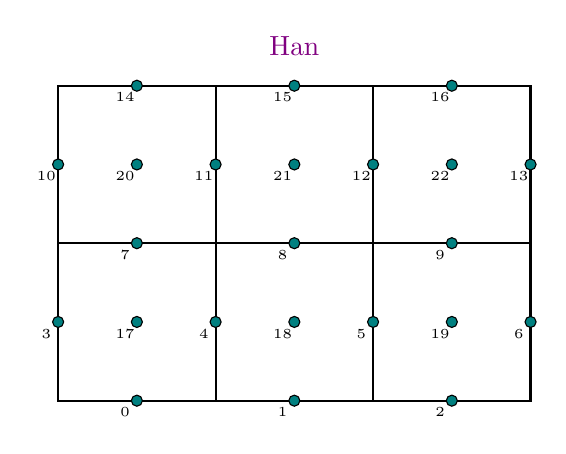
\begin{tikzpicture} 
\node[violet] at (3,4.5) {Han}; 
\draw[thick] (0,0) -- (6,0) -- (6,4) -- (0,4) -- cycle; 
\draw[thick] (0,2) -- (6,2) ; 
\draw[thick] (2,0) -- (2,4) ; 
\draw[thick] (4,0) -- (4,4) ; 
\draw[black,fill=teal] ( 1.000000 , 0.000000)     circle (2pt); 
\node[] at ( 0.850000, -0.150000 ) {\tiny 0 }; 
\draw[black,fill=teal] ( 3.000000 , 0.000000)     circle (2pt); 
\node[] at ( 2.850000, -0.150000 ) {\tiny 1 }; 
\draw[black,fill=teal] ( 5.000000 , 0.000000)     circle (2pt); 
\node[] at ( 4.850000, -0.150000 ) {\tiny 2 }; 
\draw[black,fill=teal] ( 0.000000 , 1.000000)     circle (2pt); 
\node[] at ( -0.150000, 0.850000 ) {\tiny 3 }; 
\draw[black,fill=teal] ( 2.000000 , 1.000000)     circle (2pt); 
\node[] at ( 1.850000, 0.850000 ) {\tiny 4 }; 
\draw[black,fill=teal] ( 4.000000 , 1.000000)     circle (2pt); 
\node[] at ( 3.850000, 0.850000 ) {\tiny 5 }; 
\draw[black,fill=teal] ( 6.000000 , 1.000000)     circle (2pt); 
\node[] at ( 5.850000, 0.850000 ) {\tiny 6 }; 
\draw[black,fill=teal] ( 1.000000 , 2.000000)     circle (2pt); 
\node[] at ( 0.850000, 1.850000 ) {\tiny 7 }; 
\draw[black,fill=teal] ( 3.000000 , 2.000000)     circle (2pt); 
\node[] at ( 2.850000, 1.850000 ) {\tiny 8 }; 
\draw[black,fill=teal] ( 5.000000 , 2.000000)     circle (2pt); 
\node[] at ( 4.850000, 1.850000 ) {\tiny 9 }; 
\draw[black,fill=teal] ( 0.000000 , 3.000000)     circle (2pt); 
\node[] at ( -0.150000, 2.850000 ) {\tiny 10 }; 
\draw[black,fill=teal] ( 2.000000 , 3.000000)     circle (2pt); 
\node[] at ( 1.850000, 2.850000 ) {\tiny 11 }; 
\draw[black,fill=teal] ( 4.000000 , 3.000000)     circle (2pt); 
\node[] at ( 3.850000, 2.850000 ) {\tiny 12 }; 
\draw[black,fill=teal] ( 6.000000 , 3.000000)     circle (2pt); 
\node[] at ( 5.850000, 2.850000 ) {\tiny 13 }; 
\draw[black,fill=teal] ( 1.000000 , 4.000000)     circle (2pt); 
\node[] at ( 0.850000, 3.850000 ) {\tiny 14 }; 
\draw[black,fill=teal] ( 3.000000 , 4.000000)     circle (2pt); 
\node[] at ( 2.850000, 3.850000 ) {\tiny 15 }; 
\draw[black,fill=teal] ( 5.000000 , 4.000000)     circle (2pt); 
\node[] at ( 4.850000, 3.850000 ) {\tiny 16 }; 
\draw[black,fill=teal] ( 1.000000 , 1.000000)     circle (2pt); 
\node[] at ( 0.850000, 0.850000 ) {\tiny 17 }; 
\draw[black,fill=teal] ( 3.000000 , 1.000000)     circle (2pt); 
\node[] at ( 2.850000, 0.850000 ) {\tiny 18 }; 
\draw[black,fill=teal] ( 5.000000 , 1.000000)     circle (2pt); 
\node[] at ( 4.850000, 0.850000 ) {\tiny 19 }; 
\draw[black,fill=teal] ( 1.000000 , 3.000000)     circle (2pt); 
\node[] at ( 0.850000, 2.850000 ) {\tiny 20 }; 
\draw[black,fill=teal] ( 3.000000 , 3.000000)     circle (2pt); 
\node[] at ( 2.850000, 2.850000 ) {\tiny 21 }; 
\draw[black,fill=teal] ( 5.000000 , 3.000000)     circle (2pt); 
\node[] at ( 4.850000, 2.850000 ) {\tiny 22 }; 
\end{tikzpicture} 
\end{center} 



\end{document}
